\documentclass{article}
\usepackage[english]{babel}
\usepackage{csquotes}
\usepackage{amsmath}
\usepackage{url}
\usepackage{comment}
\usepackage[a4paper, total={6in, 10in}]{geometry}
\usepackage{gensymb}
\usepackage{graphicx}
\usepackage{hyperref}
\usepackage{subcaption}
\captionsetup[subfigure]{font={bf,small}, skip=1pt, margin=-0.25cm, singlelinecheck=false}
\captionsetup[figure]{font = {small, stretch = 1}}
\usepackage{chngcntr}
\counterwithin{figure}{section}
\counterwithin{table}{section}
\usepackage{tabularray}
\usepackage{pgffor}
\usepackage{xcolor}
\usepackage{wrapfig}
\graphicspath{{./Figures/}}
\usepackage{float}

\usepackage[
backend=bibtex,
style=authoryear,
sorting = nyt
]{biblatex}
\addbibresource{Thesis.bib}

\renewcommand{\baselinestretch}{1.5} 

\title{Simulating Transition Cells under the Transition Scale-Space Model in Spiking Neural Networks}
\author{Simen Storesund}
\date{\today}


\begin{document}
    \maketitle

    \newpage
    \section*{Acknowledgements}
    Completing a master's thesis is a test of independence, but that doesn't mean I could have done it by myself. I want to give huge thanks to Nicolai Waniek, my supervisor, for his continued interest and constructive comments throughout the project. I also want to thank him for allowing me to work on the TSS model, and for creating such an interesting model to start with. Next, I would like to thank Benjamin Dunn for cosupervising, providing constructive feedback, and to his group for letting me join their group meetings. Finally, thanks also goes to the Kavli Institute, both for the interesting work they do and for letting me have an office in their building.

    \newpage
    \tableofcontents

    \newpage
    \section*{Summary}
    In the Transition Scale-Space model, entorhinal grid cells are interpreted as highly effective transition cells, responsible for accelerating retrieval of place-sequences during navigation. Previous simulations have shown that transition cells can develop hexagonal firing fields in populations of three cells, but not more. In this work, transition cell learning was simulated in spiking neural networks using theta-phase coded inputs and delayed lateral inhibition. This produced high levels of hexagonality in populations of 13 and 23 transition cells. There is also a suggestion on how boundary vector inputs can replace place inputs, using dendritic computation in a multicompartment model, which predicts that dendrites respond to single places in an even distribution across space. This is still a work in progress. There are also unanswered questions with regards to the structure of the population activity. Lastly, a pathfinding method compatible with TSS without backpropagation is presented. In sum, this is a work in favor of the biological plausibility of the TSS model, using computational resources available in biological neural networks.

    \newpage
    \section*{Sammendrag}
    Transition Scale-Spacemodellen forklarer gitterceller i entorhinal cortex som overgangsceller, som aksellererer produksjon av stedcellesekvenser ved navigasjon. I tidligere simuleringer utviklet overgangsceller heksagonalitet i nettverk på tre celler. I dette arbeidet ble overgangsceller simulert i nevrale nettverk i kontinuerlig tid, der lokasjonsinformasjon ble gitt i fasekoder og forsinket lateral inhibering mellom overgangscellene. Dette ga høy heksagonalitet i nettverk på 13 og 23 gitterceller. I tillegg presenteres en flerseksjonsmodell av overgangsceller med dendrittiske beregninger for å erstatte stedbasert lokasjonsinformasjon med grensevektor informasjon. Resultater tyder på at overgangscelledendritter bør respondere til enkeltsteder, men jevnt fordelt i miljøet. Arbeid etterlater også åpne spørsmål om populasjonsaktivitet i overgangscellenettverk. Til slutt presenteres også en modell for produksjon av stedcellesekvenser uten å bruke bakoverpropagering. Totalt utgjør dette verket et argument i favør mulig biologisk implementasjon av TSS-modellen.  


    \newpage
    \section{Introduction}
    \subsection{Animal Navigation} \label{Animal Navigation}
    A striking observation from the technological strides made in modern time is how difficult engineering robots that are able to localize and navigate autonomously is, despite how widespread it is in the animal kingdom. It is tempting to consider the striking feats of pathfinding, like birds trekking thousands of kilometers each year, following the same routes each year, or salmon returning to their home rivers after spending their adult lives in oceans half a world away. However, just looking at rodents' ability to flexibly navigate a variety of different mazes, seemingly independent of their structure or the sensory cues that are given to them, and react appropriately to novel environments or changes, after only a short time of exploration, has been a mystery for decades \parencite{Wynn2023}.

    Studying rodent navigation in a laboratory setting initially belonged to the field of psychology, before the study of the neuron, neuroscience, was properly established. Without methods for investigating the living rodent brain, numerous studies were still conducted to determine their navigational capabilities. In the 1940s, psychologist Edward Tolman conducted numerous such experiments, leading him to a conclusion that has had ramifications for the study of the brain since. 
    
    In 1946, for instance, he set up the sunburst maze to test rodent pathfinding \parencite{Tolman1946}: rats would enter a circular room from a southern arm, and the only other exit from this room was a corridor leaving from the north. Following this exit, the rodents were taken through a twisting corridor which eventually led to a food reward, in a position that was north-east of the initial room. After doing this multiple times, learning that a food reward existed at the end of the northern corridor, the rats would enter the same hub, but with the northern arm blocked. Now, multiple other corridors had been added to the room, going in different varying directions from west, north west, north east and east. Although rats had only explored the northern pathway previously, with it blocked they preferred a corridor taking them towards the north-east. 
    
    By the looks of it, the rats were aware of the geographic direction from the circular room to the food - the conditional learning they had undergone was something more than just learning that going forward and going through the winding corridor would lead to food. In a subsequent 1948-paper, Tolman described his conclusion - the rats have a cognitive map, an internal representation of the environment that would allow them to react flexibly to changes in the environment \parencite{Tolman1948}. The more accurate this internal representation is, he argued, the better the rats would be able to navigate.

    Parallel to the development of neuroscience in the following decades, shedding light on the way cognitive maps might work in brains, the rodent's ability to navigate has been studied further. A central goal was to determine what type of sensory information rodents rely on: particularly, do they navigate well with only self-motion cues, such as vestibular or proprioceptive inputs, or do they rely on information about the external world too \parencite{Dudchenko2010}?

    Using primarily self-motion cues, path integration allows deducing current position relative to a goal based on past movements by keeping track of travelled distance and direction. This method of navigation would be highly useful: it does not rely on the presence of any external information, so it reflects the flexibility seen in animal navigation. However, if the path integration system is prone to noise or bias, it might quickly accumulate error \parencite{Cheung2007}. In an interesting study, a research group tested this in hamsters by removing them from their nest, and tracking their movement in pitch darkness \parencite{Etienne1986}. The nests would typically be located at the edge of a circular environment, and the hamsters would be placed in the center. Hamsters showed an ability to home directly towards their nest. However, if the environment was subtly rotated while the hamster was being moved, some hamsters would try to move in the direction their nest would have been in, if no rotation occurred. Others found the path to the nest right away. This indicates that at least some hamsters guessed the location of their nest without using external cues. Multiple other studies have shown that rodents can navigate and home effectively without getting external information, but experiments are also clear that this only works in a limited capacity, for humans and rodents alike \parencite{Kim2013}. If the path is too long or involves too many turns, landmarks or external information might be necessary for accurate navigation.

    However, other studies have shown that rodents also rely on visual landmarks \parencite{Dudchenko2010}. One example is a study from a radial arm maze, in which eight or more arms all meet in a central intersection. At the dead end of each arm are food rewards, and on walls outside the maze are visual cues, serving as landmarks. Normally, when subjected to such a maze, a rodent will visit each arm on average once, retrieving the food and then not returning to that arm again by accident, requiring some memory of where it has already been \parencite{Suzuki1980}. However, if the landmarks are shuffled or rotated after three food-items have been retrieved, the same accuracy is not maintained.

    Studies on animal navigation are numerous, and a series of other mazes have been popularized to test navigation. The field is rich, and the observations will not be reproduced in detail here. It does seem like rodents are able to use a multitude of senses, and both path integration and external landmarks, to tell where they are in an internal, cognitive map of the environment. They are also able to tell their position relative to their goals, and plan paths depending on blockades and new information.
    
    \subsection{The Transition Scale-Space Model} \label{TSS}
    The Transition Scale-Space (TSS) model was developed and published only a few years ago \parencite{Waniek2020}. It extends Tolman's notion of a cognitive map, and can be abstracted beyond spatial maps. However, it is readily adapted to a spatial context. At its base is the following observation: to properly navigate, an animal would benefit from two distinct cognitive maps, instead of one. One map of the world, a type of memory which represents all experienced locations, and one map of transitions, how to get from one location to a neighbor.

    In this context, the place-map only needs to contain information about isolated positions, without regard to how they are connected. The TSS model also works with the neuron as the base unit, and based on experimental evidence, the fundamental unit of the place-map is a place cell, which encodes some location in an environment. These place cells can be activated from external landmark information alone, the TSS-model posits, and a place cell can give information about the nature of the place - did the rodent previously encourage a predator when that place cell was active, or is the place cell in the middle of its nest?

    However, the TSS-model places emphasis on the second network, the transition network, which can accelerate the retrieval of place cell sequences between goal- and target places. The unit of this network is the transition cell, which remembers some set of possible spatial transitions. The transition cell could be observed in multiple ways, but there are a few ways to optimize it: for one, a transition cell should represent as many spatial transitions as possible, and secondly, it should retrieve place cell sequences as quickly as possible, so the animal needs to spend as little time as possible evaluating the best path.

    From the perspective of the TSS-model, if the rodent brain has evolved a transition network, it would be optimized. Using graph theory and propositional logic (see \cite{Waniek2018}), the TSS model reasons in the following way about this transition network: while a transition neuron should encode as many transitions as possible, it must not encode transitions to and from the same place. Consider places A, B and C that are all consecutive on a linear track, and represented by each their place cell, cell a, b and c. To get from place A to C, one must pass through place B. If a single transition cell encodes both transitions from place cell a to b as well as b to c, it might produce the unwanted place cell sequence a \(\rightarrow\) c, while the wanted sequence is a \(\rightarrow\) b \(\rightarrow\) c.

    Under this constraint, the TSS model proposes a transition cell with the following activity pattern: for one, it will represent transitions from some circular region in space, called a center-area, and transitions to an annulus surrounding this circle, called a surround-area (figure \ref{TSS_transitions}). As such, any transition from a place cell with receptive field within the center-area to a place-cell with a receptive field within the surround-area is considered a valid transition by this transition cell.

    \begin{wrapfigure}{l}{0.4\textwidth}
        \centering
        \vspace*{-0.1\linewidth}
        \includegraphics[width = 0.4\textwidth]{TSS_transitions.png}
        \vspace*{-0.15\linewidth}
        \caption{Illustration of single center/surround region of transition cell. The transition cell should encode all spatial transitions from within the central circle (center area) to the surrounding annulus (surround area) as indicated by arrows. Adapted from \cite{Waniek2023}.}
        \label{TSS_transitions}
    \end{wrapfigure}

    On top of this, the transition cell will try to bundle as many of these center-surround-complexes into an environment as possible, as long as the surround-area of one complex is not overlapping the center-area of another.

    The transition cell would be active in any of the center areas, to give information about which places exist in the surrounding area. With this activity pattern, and optimally placed center-surround complexes, the transition cell would be active in a hexagonal pattern across the environment \parencite{Waniek2018,Kunsch2005}. Due to its periodicity, only three transition cells are necessary to make sure that all places in all environments are covered by a transition cell's center-area. 
    
    In any given position, a place cell will be active, giving information about current position, and some number of transition cells will be active, giving information about places in the surround area.

    In further work, Waniek determined that transition cells should operate under different scales, in which each scale represents the size of the center-surround regions \parencite{Waniek2020}. This would accelerate the rate of producing place-sequences, which was another optimization for the transition network. To accelerate sequence-retrieval, having multiple scales with increments of \(\sqrt{2}\) from one scale to the next was shown to be optimal. An estimated 7 - 9 scales would cover all behaviorally relevant scales.

    As mentioned, this model can be seen as a conceptual extension to Tolman's cognitive map: a single map isn't ideal, because both the localization information and the relational information should be stored. As will be shown in the upcoming section, the TSS model was also based on a large experimental body of observations of the rodent brain that has been found since Tolman. With this basis, the TSS-model shows that by splitting the localization- and relation-networks in two, the relational memory can both optimally accelerate finding sequences in the place-network while consisting of a finite number of highly efficient transition cells.

    \subsection{Spatial Cell Types in the Hippocampal Area} \label{Spatial Cell}
    
    \subsubsection{Place cells} \label{place cells}
    Around the same time Tolman published his thoughts the cognitive ma, the cellular unit of the brain was characterized - the spiking neuron \parencite{Hodgkin1952}. Neurons receive inputs from other neurons in rich dendritic trees, and these inputs are converted to membrane voltage potentials in the neuron. If the voltage exceeds a threshold, the neuron's axon depolarizes in an all-or-nothing action potential, making the neuron release an output of its own. These outputs are typically transmitted to other neurons over synapses.

    This formed the foundation of neurons as we understand them today. In 1971 a link between the neuron and Tolman's cognitive map was established in the place cell \parencite{OKeefe1971,OKeefe1976}. This cell was found in the hippocampus, a part of the brain initially studied due to its relevance in episodic memory. The place cell had one striking feature - while the mouse studied ran around in a square box, the cell would only be active if the mouse was within some region of the box. Seemingly, the place cell had a single preferred location in the box, and the closer the animal was to that place, the higher its firing frequency would be. Located in a part of the brain associated with memory and memory formation, it was a good candidate for a unit in a cognitive map. It has been the object of intense study since, leading to numerous important observations.

    The hippocampus is subdivided into different regions, in which three have received most attention: the dentate gyrus, CA3 and CA1 \parencite{Cherubini2015}. The dentate gyrus receives inputs from outside the hippocampus, downstream of numerous sensory modalities. The CA3-region receives inputs from the dentate gyrus, and is also heavily recurrently connected, while also providing input to CA1. CA1 gives outputs to the subiculum, which is outside the hippocampus proper and communicates with the prefrontal cortex. This pathway is called the trisynaptic circuit, and was long thought to be the dominating one for hippocampal activity. Place cells have been found in both CA3 and CA1, showing similar properties. Curiously, place cells have not been found in other brain areas, and additionally, severing the connection from CA3 to CA1 does not diminish CA1 place cell activity significantly \parencite{Brun2002}.

    Within CA3 and CA1, only a fraction of the cells will behave as place cells in some environment. However, as a population, these cells can cover the environment, making the foundation of a spatial cognitive map \parencite{Wilson1993}. Moreover, upon changing environments, the networks undergo orthogonal, global remapping - some place cells will remain as place cells, others will not, and there seems to be no correlation between the places they occupy in one environment and another \parencite{Muller1987}. If the environment is changed, such as changing the color on the walls, some place cells might remap, others might not - partial remapping. This seems to imply that place cell activity is somehow context dependent, although the cause and purpose of this is unknown.

    The hippocampus and surrounding regions exhibit oscillatory local field potentials during locomotion \parencite{Winson1978}. The periodicity is typically between 4 and 11 Hz, and place cell activity has been found to depend on the phase of this wave \parencite{OKeefe1993,Skaggs1996, Hafting2008}. During locomotion, the place cell that is most active in the current position will activate at the trough of the theta phase, a place cell whose most active position was recently passed will activate a little earlier, and a place cell whose most active position will shortly arrive will activate a little later - in the descending or ascending parts of the theta cycle, correspondingly.

    This phenomenon, called theta phase precession, shows that the phase-timing of the place cell gives some information about the time the animal will reach that place, but it also leads to preplay \parencite{Dragoi2011,Dragoi2013}. The way place cells activate relate to phase means that each theta-cycle, a short sequence of place cells will activate consecutively, starting with place cells representing places the animals just were, and ending with place cells its shortly going to arrive at.

    A separate phenomenon was discovered before preplay, called replay, and occurs during sleep or rest after navigation \parencite{Wilson1994,Olafsdottir2016}. In the study that first discovered this, the animal ran along a track, so the same sequence of place cells activated repeatedly. Following this, during sleep, the same sequence was replayed, forwards and backwards, but compressed significantly in time. Curiously, reverse replay is seen more frequently after increasing reward \parencite{Ambrosa2013}.

    This establishes the networks of hippocampal place cells as an interesting option for a cognitive map of the rodent's spatial environment. The remapping, theta phase precession and replay are some of its distinguishing features, implying that the network both has some concept of context and of spatial sequences. However, it is not clear what neural inputs the place cell uses to compute place fields, or what causes remapping. One brain area of interest in this context was the hippocampus' main input structure - the entorhinal cortex. In this region, multiple spatially modulated neurons have since been found, the most striking of which might be the grid cell.

    \subsubsection{Grid Cells} \label{grid cells}
    When looking for other cells with spatial signatures, next to the place cell, the entorhinal cortex was a candidate as the main input structure to the hippocampus. In 2004, this led to the discovery of the grid cell, a cell which fires periodically in space in a hexagonal lattice \parencite{Hafting2005}. While place cells early were recognized as a possible component in a cognitive map, grid cells did not immediately fit into existing frameworks of cognition. Since their discovery, numerous studies have shed light on their features, but their purpose and function is still unclear. 

    Grid cells were first found in the second layer of the medial entorhinal cortex (mECII) but have since been found in the third and fifth layer (mECIII and mECV), as well as in the pre- and para-subiculum \parencite{Boccara2010}. In the mECII, hexagonal activity has been observed in both stellate and pyramidal principal cells \parencite{Rowland2018}.
    
    The hexagonal acivity pattern of gridcells differs in three primary variables between grid cells - the scale of the grid, its orientation relative to the environment and its phase. Grid cells in mECII that are physically close tend to have similar scale, orientation and phase \parencite{Hafting2005}. In square environments, grid cells typically coalign with a 7.5 degree orientation offset relative to one environment wall. Meanwhile, grid cell scale seems to increase discretely and geometrically in grid cells along the dorsoventral axis, increasing by a factor between 1.4 and 1.7 from one scale to the next \parencite{Stensola2012}. This indicates that grid cells belong to modules, in which all cells within a module share orientation and scale, but scale varies between modules. Within a module, grid cells have varying degrees of firing field overlap, depending on their phases.

    On a whole, grid cells firing fields are noted for their robustness - their firing field is maintained in the absence of sensory inputs, indicating a measure of path integration, and firing in pure grid cells is independent on animal velocity and heading direction \parencite{Hafting2005}. While they show theta phase precession similar to hippocampal place cells, they do not remap orthogonally, as grid cells maintain their relative orientation, phase and scale compared to other grid cells in the network when environments change \parencite{Hafting2008, Fyhn2007}. 

    Curiously, grid cells' firing fields have been noted to not always be perfectly hexagonal: shearing effects that seem to curve the grid have been observed in sufficiently large square environments or in environments with non-regular shape (maybe hone this?) \parencite{Stensola2015,Krupic2015}.

    Topological analysis has captured these features in the population activity across a grid cell module \parencite{Gardner2022}. In narrow time windows, the grid cell population firing can be placed on the manifold of a twisted torus. This indicates that across environments, and regardless of environmental shape or shearing effects, the network is somehow organized so the correlation between two grid cells spiking is maintained, and organizes onto a two-dimensional toroidal surface for the entire module.

    The mECII receives inputs from large regions of the brain, but the most notable are neighboring regions CA1, the pre- and parasubiculum, the retrosplenial cortex as well as the post- and perirhinal cortices \parencite{Kerr2007}. Lesioning inputs from CA1 has been seen to impair grid cell activity, showing important connectivity from CA1 \parencite{Bonnevie2013}. However, as CA1 is downstream of the entorhinal cortex, both directly from mECIII and indirectly via the trisynaptic pathway from mECII, this might not be a satisfactory input structure providing grid cells with spatial information \parencite{Tamamaki1993,Kerr2007,Witter2017}.

    It is not clear how the other main input structures impact grid cells, but in rodents, removing the theta oscillations by disabling the medial septum impaired the hexagonal field \parencite{Brandon2011,Koenig2011}. Curiously, grid cells maintained normal firing without theta oscillations in bats \parencite{Yartsev2011}. More than this, the post- and perirhinal cortices are known to integrate numerous sensory modalities, and multiple spatially modulated neuronal types have been observed in the pre- and parasubiculum, so these might provide spatially modulated sensory inputs to grid cells \parencite{Furtak2007,Groen1990}. Although \cite{Hafting2005} found stable gridness in darkness in rats, \cite{Chen2016} tested gridness in darkness in mice, and found this to be disrupted leading to the conclusion that visual stimulus indeed is important for maintaining grid fields.

    In terms of output, mECII grid cells have not been observed to be excitatory recurrently connected. However, multiple studies have confirmed a fast-acting lateral inhibition within mECII by parvalbumin-positive interneurons \parencite{Couey2013,Buetfering2014}. Maturation of this interneuron layer during development strengthens the grid pattern \parencite{Christensen2021}, indicating that these lateral connections are important for the grid field.

    The purpose of grid cells is widely discussed, but a few candidates have been suggested. Because the mEC gives inputs to the hippocampus, it was speculated if multiple grid cell modules together could produce place cell activity. However, place cell dependence on grid cells was disproved when grid cells were shown to develop later in development than place cells (postnatal day 16-17 vs 19-20) \parencite{Langston2010,Wills2010,Wills2012}.

    Because grid cell firing is maintained in darkness, a suggested function has been path integration, which would indicate that grid cell activity would mostly be predicated on velocity information. Other models, such as the TSS, suggest that grid cells participate in navigation by integrating external sensory information. The striking, hexagonal firing fields, as well as the unclear purpose, has lead to a series of different computational models that focus on different grid cell properties, that will be reviewed in section \ref{Grid Models}.

    \subsubsection{Other Spatially Modulated Cells}
    Grid- and place cells both have striking firing fields, but they are by no means the only cells that have been found showing some spatial preference. This section will briefly mention some of the others, focusing on their activity pattern and location in the brain.
    
    All the following cell types have been found in the parahippocampal area, including the entorhinal cortex, subiculum and pre/parasubiculum, but not the hippocampus, and are functionally defined \parencite{Brandon2014}. The first of these, the head direction (HD) cell, was first found in 1990 in the parasubiculum, and was since also found in the presubiculum and mEC layer III and V, but, interestingly, not in layer II \parencite{Taube1990}. The HD cell is active independently on the animal's position in an environment, but fires preferentially when the head is turned a given direction - collectively, a population of HD cells can encode all head directions. Pathways giving rise to HD cells have been established, showing that vestibular input is critical for their activity, aided by prioprioception and external senses \parencite{Taube2007}. Conjunctive cells have been found in the same brain areas, firing preferentially if the animal is simultaneously on a hexagonal grid and facing a given direction \parencite{Sargolini2006}. These conjunctive cells have also not been found in mECII.

    Combined with the head direction cells, finding the speed cell showed that there is velocity information present in the entorhinal cortex, as necessary for path-integration \parencite{Kropff2015}. These speed cells were found across all layers of the mEC, and the spiking of a cell correlated highly with the animal's future speed 50 - 80 ms in the future.

    Boundary vector cells and border cells have been found across all layers of the mEC, as well as in the pre- and parasubiculum and the subiculum \parencite{Solstad2008,Boccara2010, Lever2009}. These cells are preferentially active when an environment boundary or border is in some preferred direction - border cells when the boundary is immediately next to the animal, boundary vector cells if the boundary is at some fixed, preferred distance. Recent findings suggest that boundary vector cells in the subiculum alter activity based on environment geometry, aligning with candinal directions in square environments but not in circular \parencite{Muessig2024}. Another type of vector-based spatially modulated cell is the object vector cell, which activates if some environment landmark is both in some preferred direction and distance \parencite{Høydal2019}.

    Modelling work has shown that boundary vector cells can get their receptive fields to high precision using optic flow \parencite{Raudies2012}. The similarity between the models for head direction cells and this one is that they don't depend on prior knowledge of the environment to explain the cellular activity. This makes them viable candidates as providing spatially modulated information to other cells, such as grid cells or place cells, during exploration.

    \subsection{Existing Grid Cell Models} \label{Grid Models}
    A multitude of models and model families already exist to explain the wealth of experimental data on grid cells, with differences in their suggested mechanisms for the grid pattern, as well as the purpose of the grid cell. Due to their persistent spiking in darkness, many models assume that grid cells path integrate, accumulating self-movement information to predict current location in the absence of external input. Oscillatory interference (OI) - models seek to explain the theta phase precession in grid cells, and have shown that grid-like activity can be achieved by the interference of multiple oscillators in a cell's membrane potential \parencite{Burgess2007,Zilli2010}. The OI-model can account for many activity patterns besides the hexagonal grid, but if the different oscillators differ in frequency by a sufficiently small margin, and adapt this based on velocity-inputs, the cell can have a grid-cell-like activity with spacings as observed in experiments. Since the theta oscillations typically is one of the interfering oscillations in OI-models, these models reproduce observations of both theta phase precession and the impaired grid cell firing when theta oscillations are disrupted.

    Another set of models suggest grid cells as part of a continuous attractor network (CAN), which can explain persistent grid cell activity during rest or sleep \parencite{Yoon2013,Widloski2014}. These models have been implemented with lateral inhibition between grid cells, as observed in mECII \parencite{Couey2013}, as long as the strength of the inhibition is inversely proportional to the overlap of firing fields, so the most active grid cell silences all other grid cells. When the animal moves, this activity is shifted to a grid cell with a neighboring phase. This CAN-model has been supported by the topological analysis of mECII-activity by \cite{Gardner2022}, and gained traction in recent years \parencite{Sorscher2023}. It has been demonstrated that any such system of path integration still needs regular external input to avoid drift \parencite{Cheung2007, Mulas2016}, and the exact inhibitory structure predicted by CAN - networks has not been observed \parencite{Zilli2012}. 

    A third group of models predict that grid-patterns can be learnt by Hebbian learning, in which grid cells get their firing fields by associating to suitable spatial inputs and dissociating from other spatial inputs \parencite{Soldatkina2021}. As opposed to the OI- and CAN-models, the driving mechanism of grid cell activity in these feed-forward models is not necessarily self-motion inputs, but that doesn't exclude the possibility that grid cells play a role in path integration. An early idea was to model grid cells with firing fatigue and place cell-like input activity, which was not necessarily hippocampal place cells \parencite{Kropff2008}. In this model, there were two primary factors for learning - competitive firing rates between grid cells, so the total population firing rates were normalized, as well as a firing fatigue, so the current firing rate would be negatively influenced by prolonged high past rates. Grid cells would then associate to place cell inputs based on their mutual firing, and the fatigue prevented the same grid cell from associaing to all inputs. While this produced grid like cells, carefully tuned excitatory collaterals between gridcells were necessary to make them share orientation.
    Later, this excitatory collateral was replaced by inputs from a layer of collateral cells that received both place cell-input and head direction-cell input, so the model produced grid cells with shared orientation in a purely self-organized manner \parencite{Si2013}.

    Some models generate grid cells with a center-surround learning rule from place-cell inputs. In these models, grid cells typically associate to place cell inputs with firing fields within a center-area, and dissociate from place cells with firing fields in an annulus around this area. \cite{Mercado2020} showed that this learning rule, combined with lateral inhibition, reduced boundary-effects on grid formation and gave a high level of gridness. While the grid cells prefered an orientation around 7.5 degrees relative to the walls in a rectangular environment, in line with experimental results, all grid cells were found in one of three distinct phases. Another feedforward model added a second annulus around the center-surround area, and place cells within this narrow ring were tagged so that new firing fields could only be placed on this \parencite{Castro2014}. Moreover, if a place cell would get tagged from two separate firing fields of one grid cell, the weights would potentiate. While this was robust to noise, it is unclear if orientations and phases would align between grid cell.

    \subsection{Grid Cells as Potential Transition Neurons} \label{Grid cell as Transition cell}
    In line with the current models, TSS proposes place cells as units in a cognitive map of the environment \parencite{Waniek2018}. The place cell learns to activate based on spatially modulated sensory inputs, in which each place cell associates to spatial inputs from one area, and lateral inhibition prevents other place cells from activating. This has been explored in models, for instance using boundary vector cells as inputs \parencite{Barry2006}. 
   
    The grid cells are suggested as TSS transition cells, collectively forming a transition network. As predicted for transition cells, grid cells typically have a hexagonal activity, and are divided in modules based on their scale, incrementing by a factor close to the \(\sqrt{2}\), optimal to accelerate sequence retrieval.

    To learn these firing fields, TSS posits that transition cells correlate and decorrelate to the same spatial inputs as place cells. As opposed to place cells, transition cells associate to spatial inputs responding to center-regions, and dissociate from inputs in the surrounding-regions, while trying to fit as many center-regions into the environment as possible. This resembles some of the feed-forward models presented above. Similarly to CAN-models, however, TSS suggests that transition cells are interconnected by strong lateral inhibition, to discourage overlapping center-regions.
    
    The connectivity between the place cell network and the transition cell network that enables flexible path-planning is then learnt on top of this, based on correlated place- and transition cell activity.

    A learning rule for transition cells has been shown to produce grid cell-like transition cells in discrete-time simulations. In these simulations, transition cell networks consisted of three transition cells, the smallest possible number to cover the entire environment, and the transition cells received place-like inputs sampled from a regular, rectangular grid of spatial afferents \parencite{Waniek2017}. In discrete time-steps, activity in the spatial cell layer would activate transition cells depending on a position in a simulated trajectory. Following this, three separate learning rules would update input-to-transition cell weights. The first rule would let the most active transition cell associate to the central spatial cells, and dissociate from surronding spatial cells. The second rule, called the baseline, would increase the weights from the active input cells to all transition cells, for both active and inactive transition cells. Third, an interaction rule would weaken the connection from inputs to all transition cells except the most active one.
    A rationale for the three learning rules is that the first rule provides the center-surround effect necessary for transitions, the baseline encourages transition cells to be active as frequently as possible to encourage effective transition cells, and the interaction rule discourages excessive overlap between transition areas.
    
    Although this network gave cells with high gridness in networks of three transition cells, it was not explored in bigger networks. Additionally, it is unlikely that a biological network providing the spatial inputs shows regularly distributed, place like activity, at least prior to exploring the environment. Both of these constraints need to be addressed for the TSS model to be considered biologically plausible.

    \subsection{Thesis Goal} \label{Thesis Goal}
    In this work, the main objective is to build upon the simulations already conducted in the TSS-model, with the aim to 1) establish this network structure in a more biologically plausible way, and 2) explore under what conditions or constraints transition cells develop a hexagonal structure.

    Following this aim, the objective is split into two paths. First, to see if a biologically plausible network can contain more than three grid cells, by simulating continuous time with delayed inhibition. The hypothesis is that this delayed inhibition allows multiple transition cells to develop gridness by partly overlapping their firing fields. The network should resemble the previous simulation as much as possible, to allow some level of comparison.

    Second, the way the structure of spatial input affects gridness is also explored. This is both to see if using rectangularly spaced inputs is necessary to produce gridness, and to evaluate the possibility of vector-based inputs such as BVCs, instead of place-like inputs.

    With a simple STDP- based learning rule, along with a baseline weight modulation, transition cells developed high gridness levels in larger networks than previously observed, and in with multiple network structures. This is an argument that cells can learn spatial transitions effectively under biologically plausible conditions. However, gridness did not occur in models with BVC-inputs, and it is unclear if this is because of the overall model design or the choice of hyperparameters.
    
    \newpage
    \section{Methods} \label{Methods}
    \subsection{Overall model design} \label{Overall Method}
    This thesis seeks to test gridness in transition neurons as described by the TSS-model with biologically plausible conditions. To achieve this, transition cells were simulated in a spiking neural network, which are artificial neural networks with certain properties:
    \begin{enumerate}
        \item The network is simulated in continuous time, or with time steps that are vastly shorter than the mean firing rate of neurons.
        \item Neurons communicate in temporally discrete spikes, triggered when an internal voltage variable exceeds a threshold.
    \end{enumerate}

    In addition to these properties, an ideal network must meet more requirements to be considered biologically plausible in this work. First, all communication should happen at a temporal delay. Second, learning rules must be online and local. Online and local learning rules mean that all variables necessary for learning must be available at the time of learning (online) and in the physical location where learning occurs, typically the synapse (local) \parencite{VanDerVeen2022}. 
    
    Spike timing dependent plasticity (STDP) is a learning rule in which a synapse updates weights both when the presynaptic and the postsynaptic neuron spikes \parencite{Song2000}. The weight-update is according to a STDP-kernel, in which weights are decreased upon presynaptic activity and increased on postsynaptic activity. The magnitude of weight decrease is high if there was a postsynaptic spike shortly before the presynaptic inputs, and the magnitude of weight increase is high if there was a presynaptic spike shortly before postsynaptic activity. The processes of decreasing and increasing weights do not need to be symmetric. By the conditions above, STDP is a biologically plausible learning rule.

    A baseline learning rule increments weights slightly when a presynaptic neuron is active, regardless of postsynaptic activity. This learning rule is also online and local, satisfying all constraints.
    
    Next, an ideal network should get inputs from some plausible spatially tuned neuron type, more precisely boundary vector cells (BVCs), whose activity is based on real or simulated trajectory data \parencite{Lever2009}. From these inputs, another layer of cells of arbitrary size learns center- and surrounding area information to represent transition-cells as described in the TSS-model, encoding transitions on a single scale. The reason BVCs are considered plausible is that their activity can be maintained even when exploring novel environments (see \cite{Raudies2012}).
    
    Finally, an ideal network is not dependent on highly specific parameters, and shows some robustness to noise, which is likely necessary for any actual brain network.

    Under these constraints for plausibility, the aim of the work is to test whether transition neurons self-organize into modules with hexagonal activity patterns in space, and if this is in line with experimental results of gridcells in the mECII, as predicted by the TSS model \parencite{Waniek2018}.

    Both an ideal network and subsequent simplifications will have some common features to accommodate these objectives: To facilitate STDP, which allows center-surround learning, all inputs arrive in pulses at theta-wave frequency set at 10 Hz, in which only spatial input with sufficient relevance is active (figure \ref{mouse_plot} (a)). The input is also phase coded, so the less relevant it is, the higher the temporal offset is relative to theta (figure \ref{mouse_plot} (b)). This means that a transition cell is likely to fire following center-inputs, and following receive a wave of inputs from cells representing surrounding locations. The STDP learning-rule will encourage potentiation of the center-activity, which arrived pre-spike, while the surround-activity arriving post-spike is depressed. Secondarily, all active inputs are slightly potentiated to encourage the transition cell to be active in as many center-areas across the environment as possible, according to a baseline-learning rule (see equations \ref{key3} and \ref{key4} for implementations).

    \begin{figure}[htbp]
        \centering
        
        \begin{minipage}[b]{0.61\textwidth}
            \centering
            \subcaption{}
            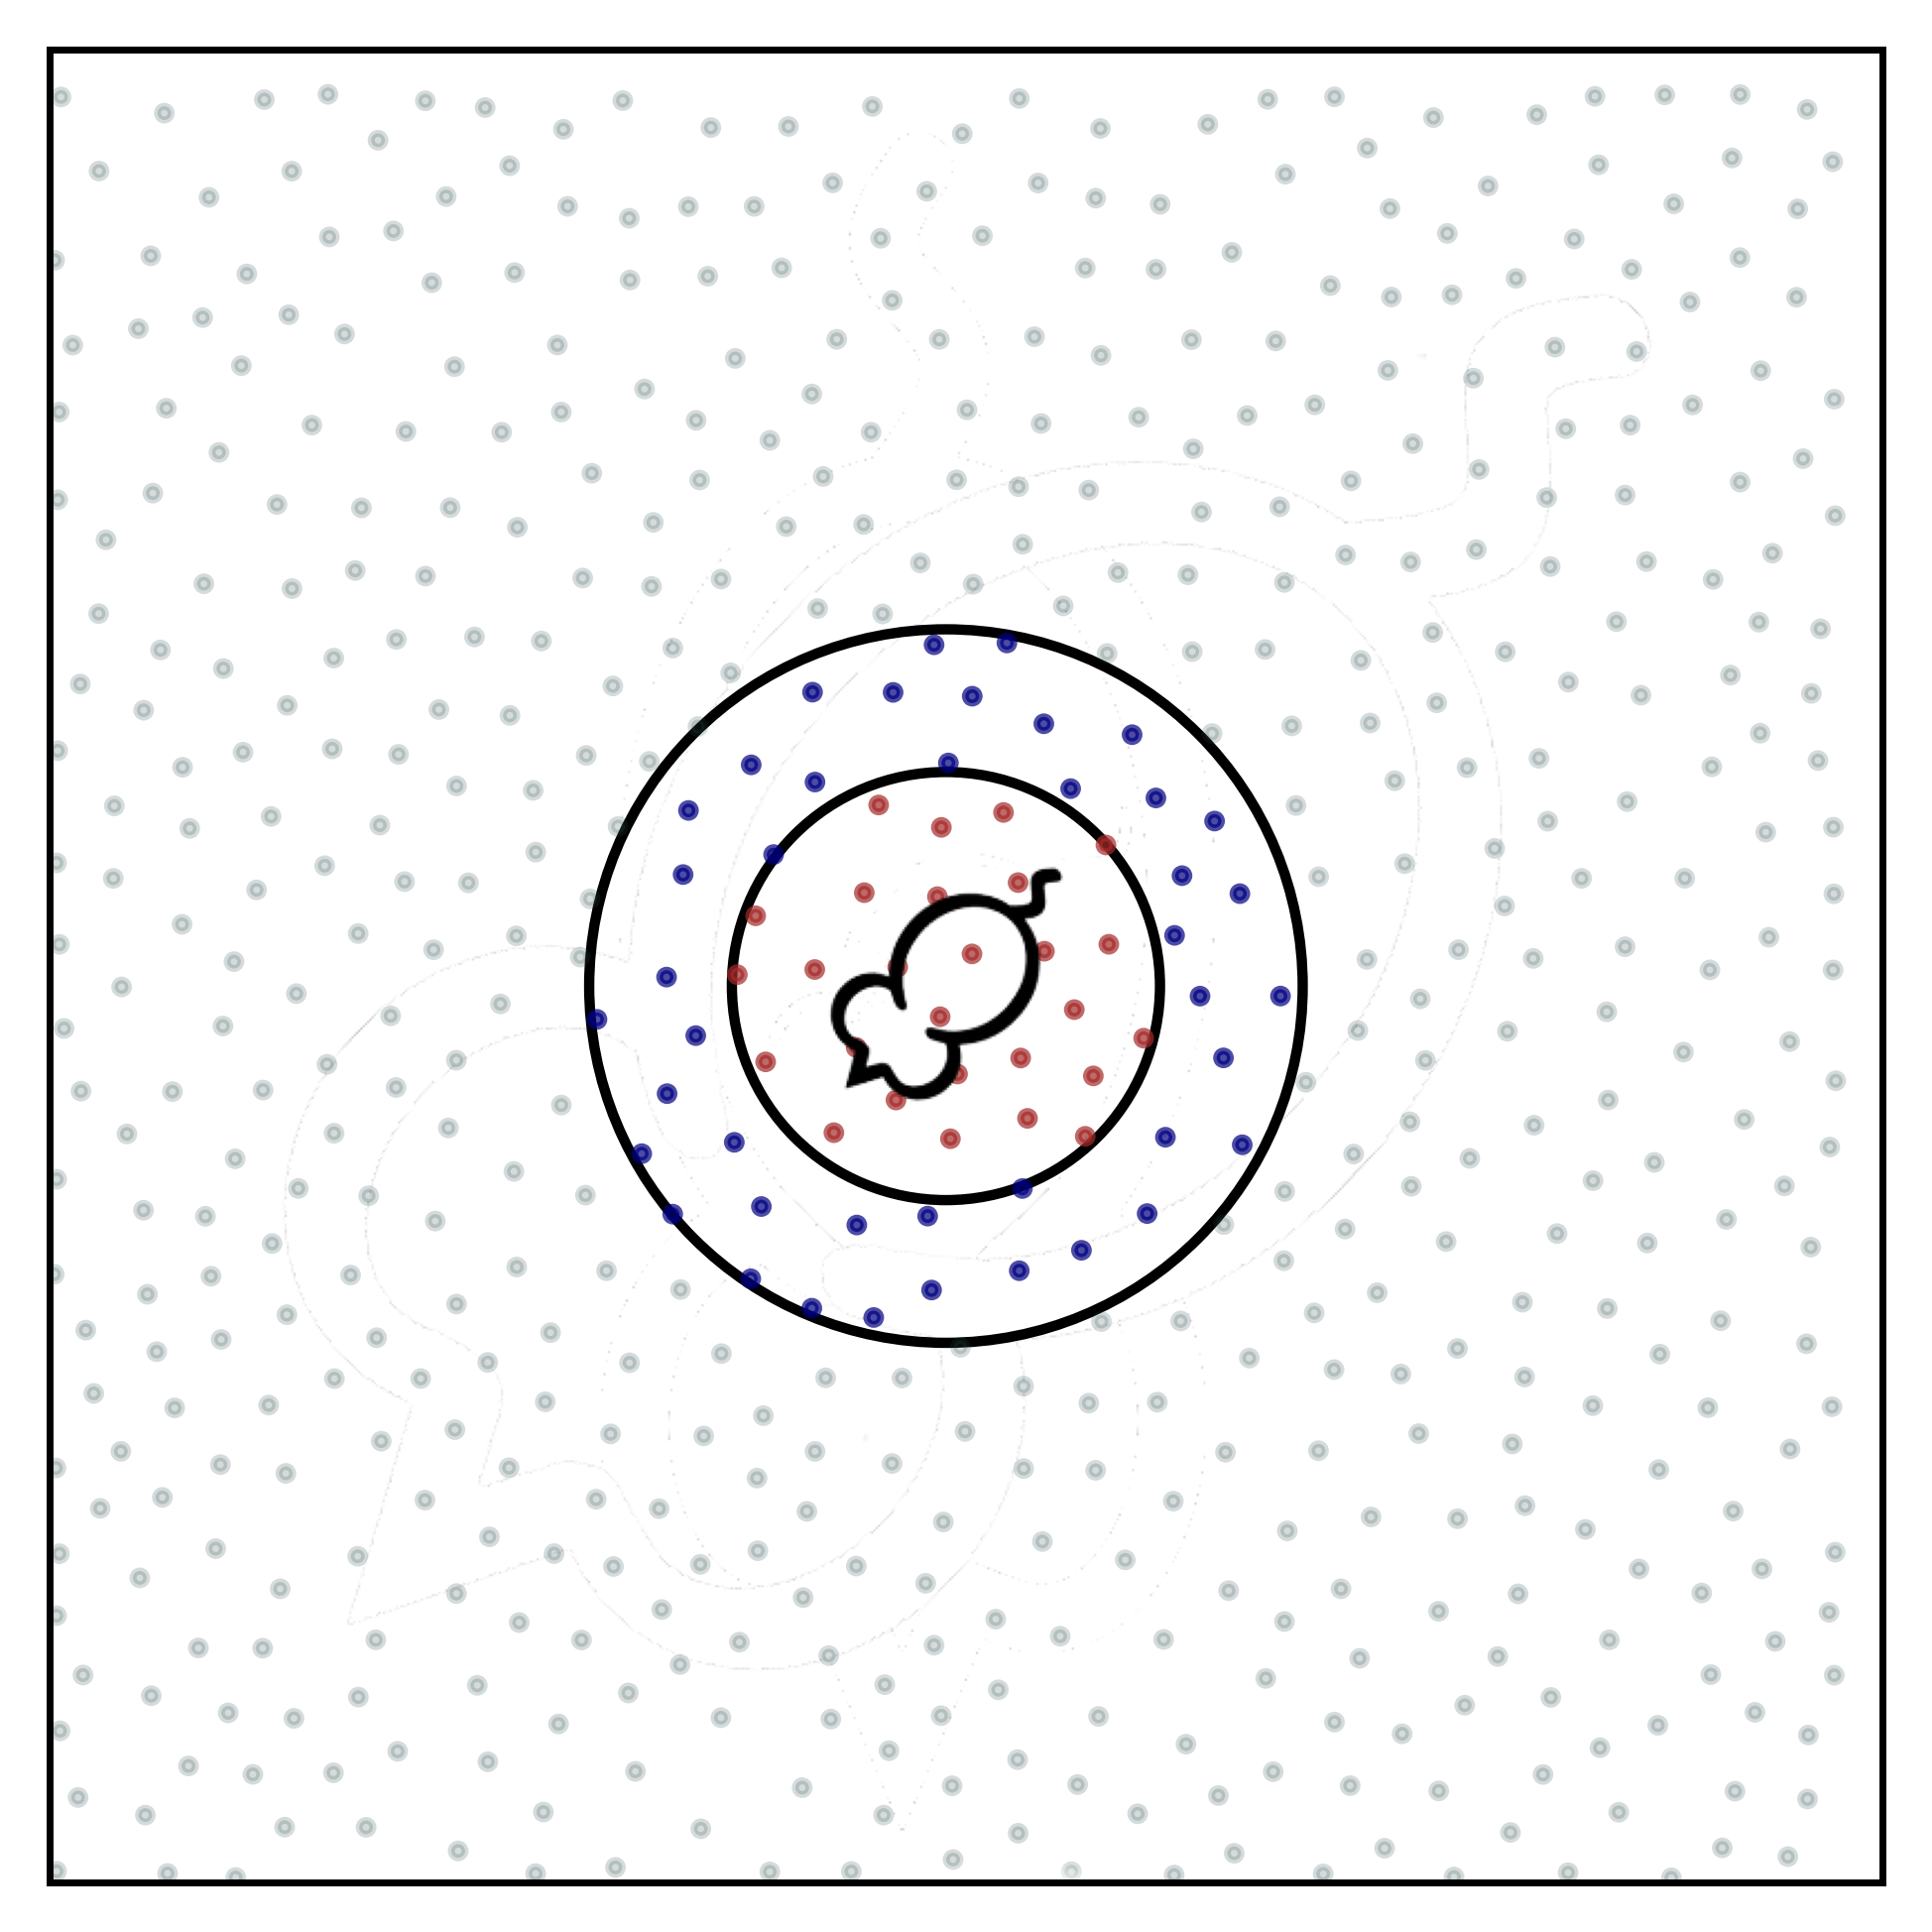
\includegraphics[width=\textwidth]{mouse_plot.png}
        \end{minipage}
        \begin{minipage}[b]{0.38\textwidth}
            \centering
            \begin{subfigure}{\textwidth}
                \subcaption{}
                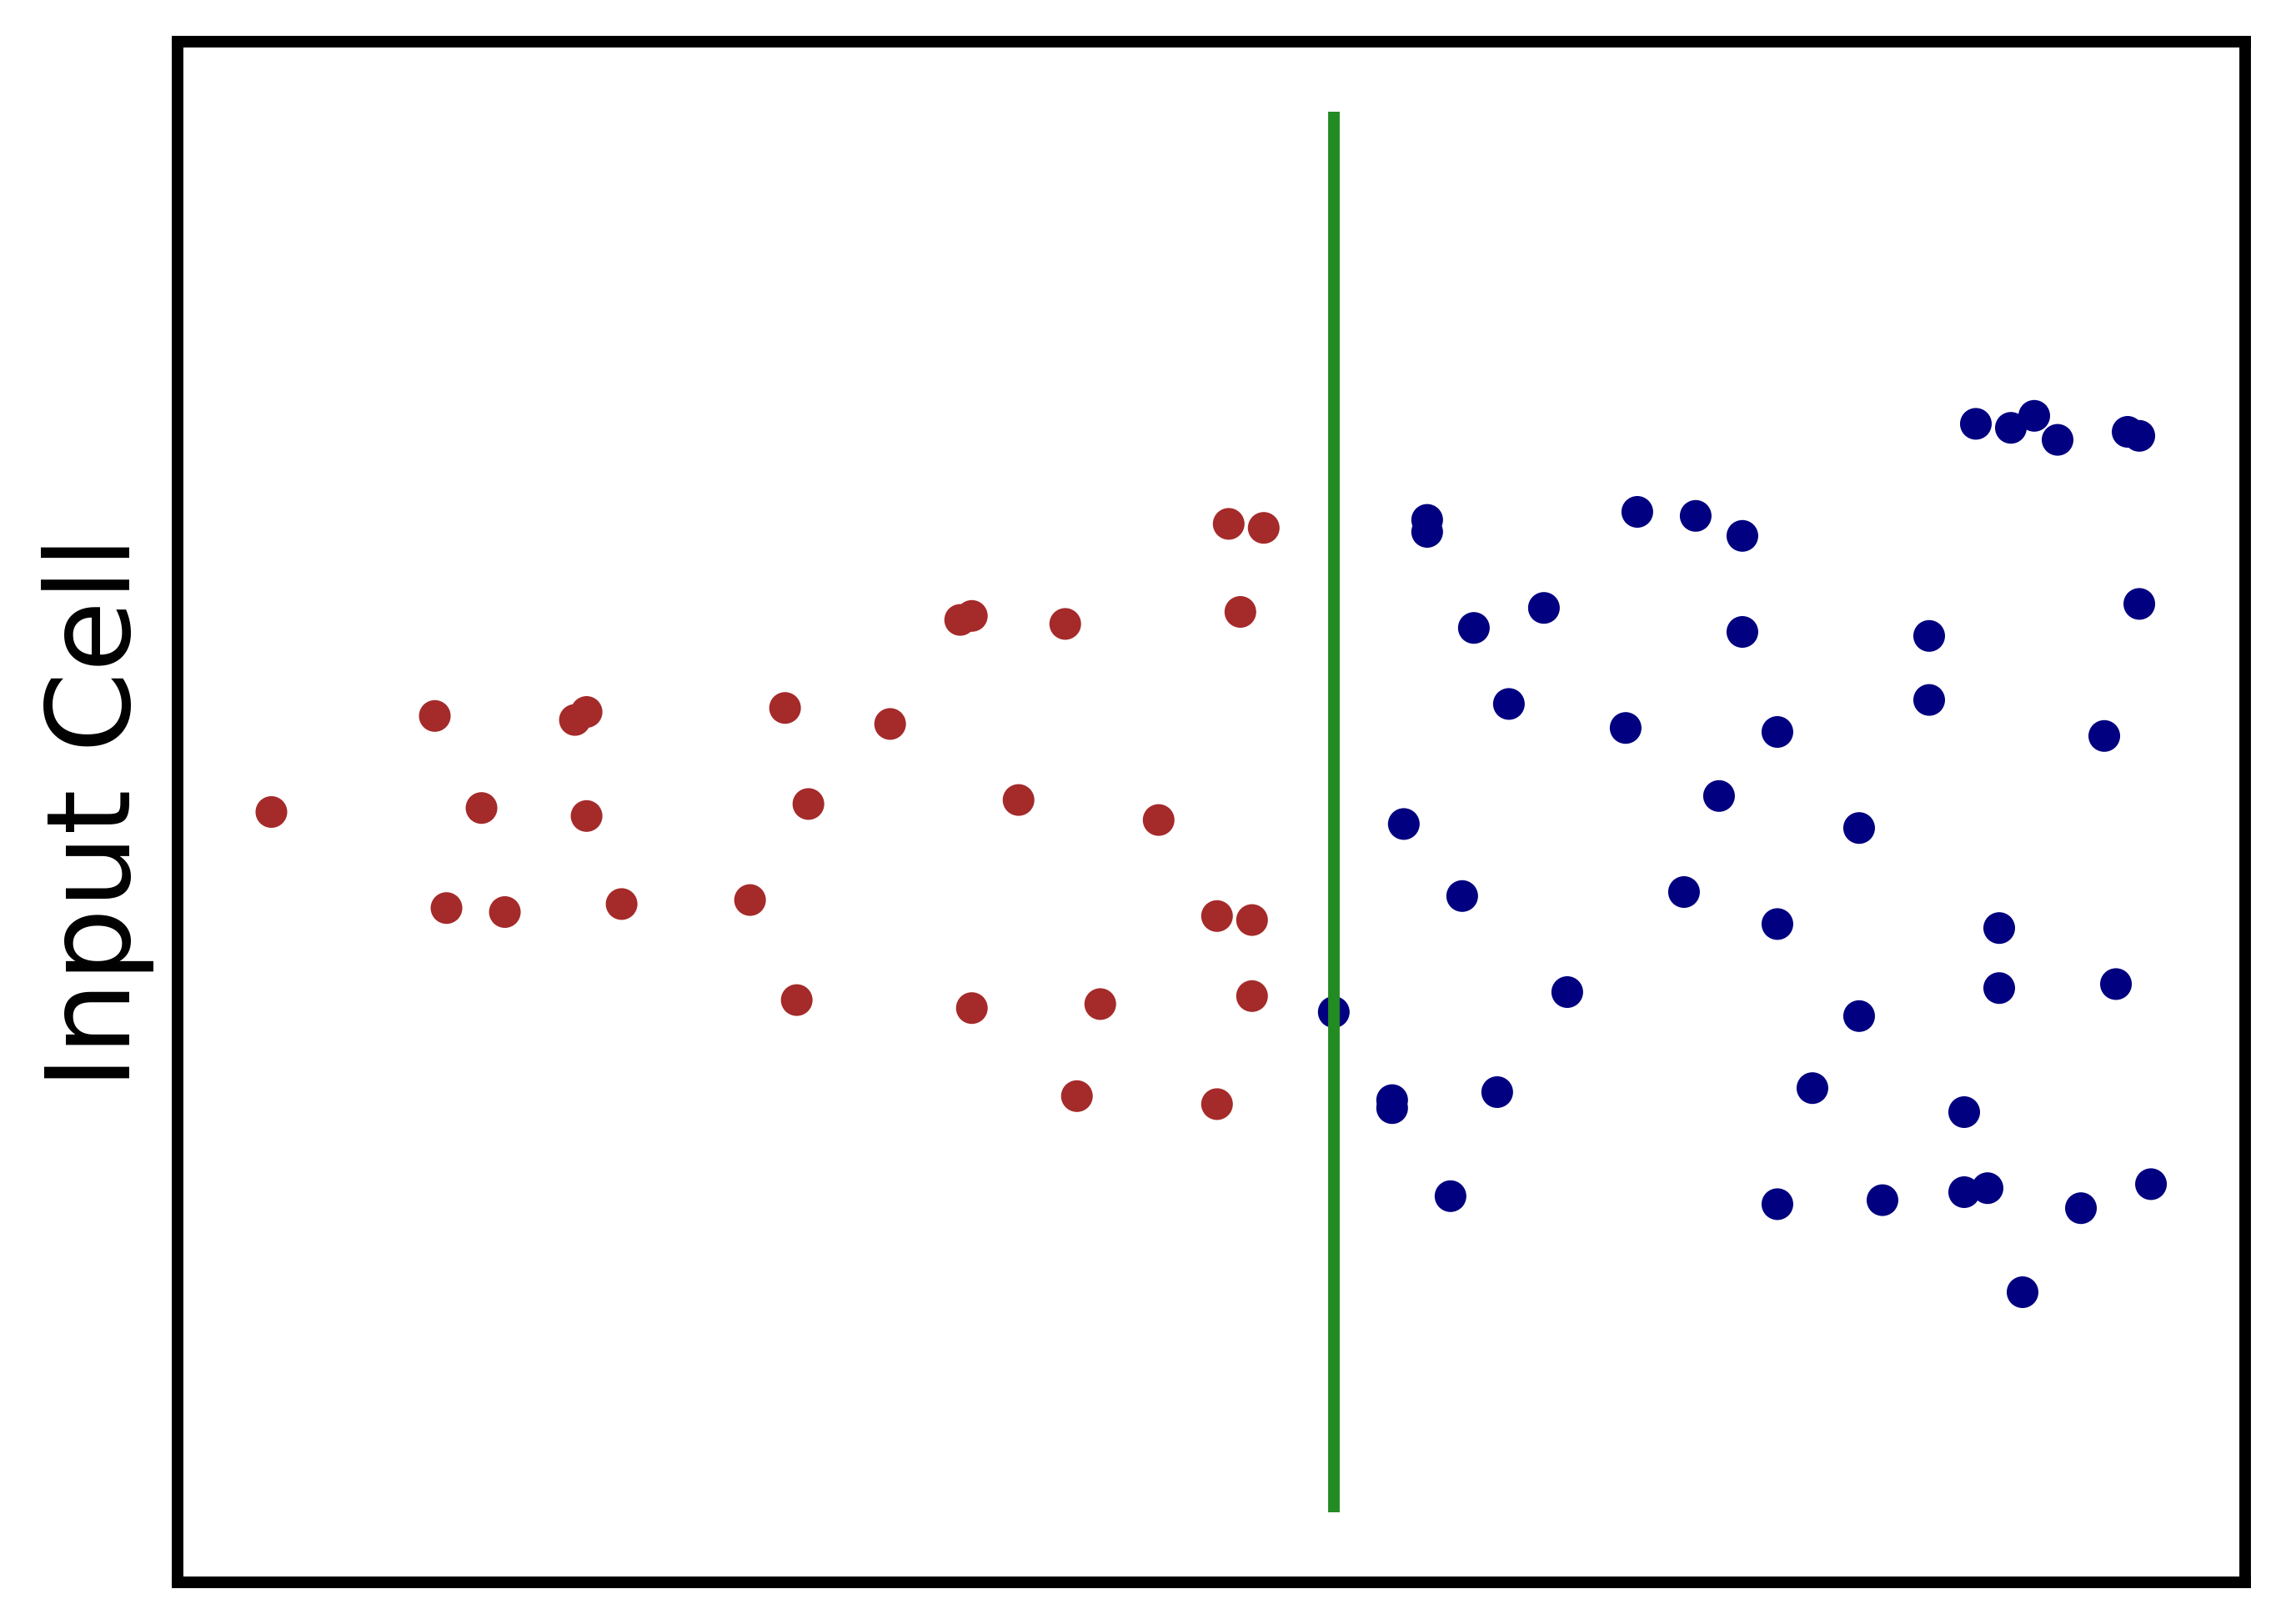
\includegraphics[width=0.95\textwidth]{input_STDP_plot.png}
            \end{subfigure}
            
            % \medskip
            
            \begin{subfigure}{\textwidth}
                \subcaption{}
                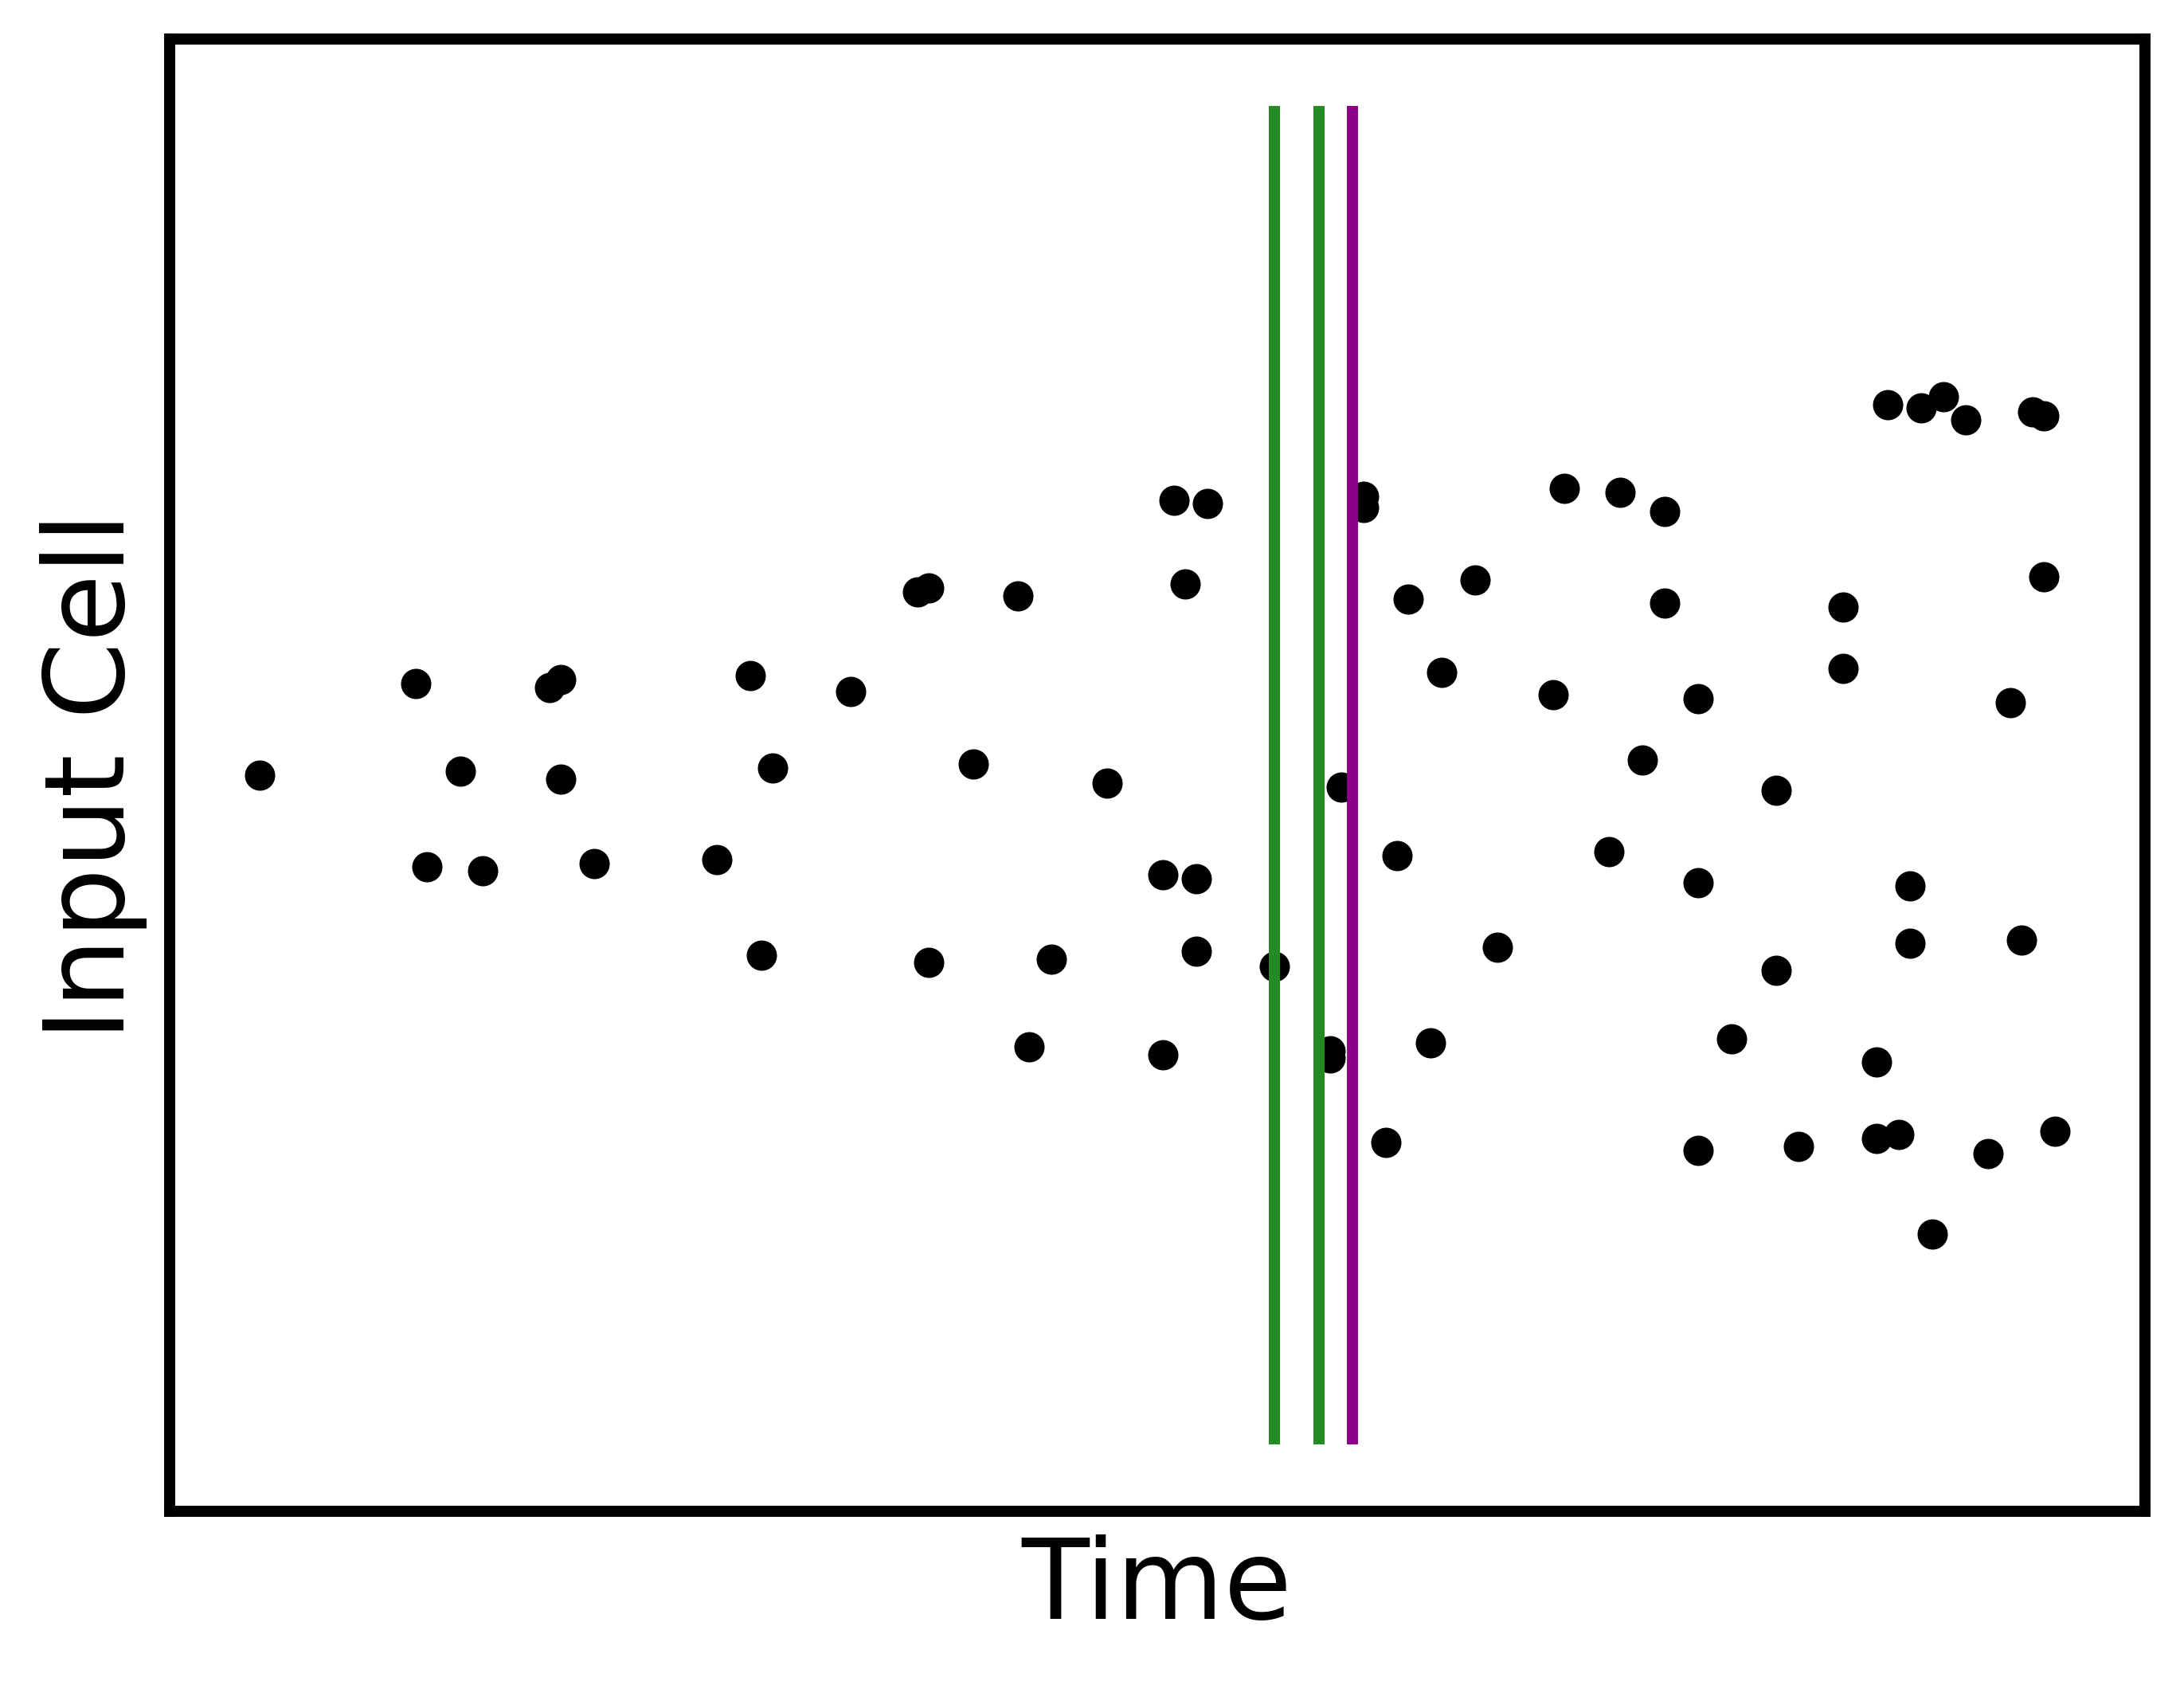
\includegraphics[width=0.95\textwidth]{input_inhibit_plot.png}
            \end{subfigure}
        \end{minipage}%
        
        \caption{The nature of phase coded spatial inputs. (a) Spatial inputs from a region surrounding the mouse will be activated each theta-cycle (10 Hz), here indicated by points within the two surrounding circles. This input is phase-coded, so cells responding to locations closest to the mouse will activate first. (b) Hypothetical raster plot showing input activity in one theta cycle. The spike time of a transition cell (green vertical line) determines which inputs the transition cell will associate to and dissociate from. In this case, the transition cell associates to the inputs colored red (left of the vertical line), and dissociate from the inputs colored blue (right of the vertical line). Comparing to the inputs' locations in (a) (color coding preserved), this can encourage center-surround learning. (c) Delayed inhibition (purple vertical line, rightmost) can allow multiple transition cells (green vertical lines, middle and left) to fire during the same theta-cycle.}
        
        \label{mouse_plot}
    \end{figure}

    An inhibitory layer connects transition cells laterally, causing strong inhibition, but on a delay. This leaves a narrow window in which multiple transition cells can fire, followed by complete inhibition in which no transition cell can fire for the remainder of the theta cycle (figure \ref{mouse_plot} (c)). The window can allow so some transition cells partially associate to the same areas.

    \subsection{Considering BVC inputs} \label{Considering BVC inputs}

    One goal of this work was to obtain grid cell-like transition cells with BVC inputs, and a way to model this is with a direct connection between the two with transition cells as leaky integrate-and-fire (LIF) neurons. In this kind of model, transition cell activity is based on linear summation of BVC inputs. There are reasons to think that such a network is difficult to achieve. The following idea explains this: in square environments, one could imagine picking two locations that the transition cell has associated to, denoted \((x_1, y_1)\) and \((x_2, y_2)\), and that should make up two firing fields in the hexagonal pattern. In locations \((x_1, y_2)\) and \((x_2, y_1)\), the input would be highly similar to half the input from position 1 and half the input from position 2, due to the nature of BVCs. Notably, though, the transition cell should not fire in these locations, because that would likely lead to rectangular grid firing patterns, not hexagonal. This would be true for all pairs of firing fields that are not parallel to one of the walls. In other words, square environments and linear summation of BVC inputs is expected to encourage rectangular fields, not hexagonal.
    
    It should be noted here that the spiking neural network itself implies non-linear features that might have enabled such a network to produce grid-cells. One way to achieve this would be with other transition cells that are sufficiently active in location \((x_1, y_2)\) and \((x_2, y_1)\), so they inhibit the first transition cell. However, due to the fine-tuning such a network would require, alternative network structures were preferred.

    One such alternative, which highlights an advantage of biological neurons over simplified artificial ones, appears after considering nonlinear dendritic computation in transition cells in a multi-compartment model. This kind of model still implies that boundary vector cells synapse onto transition cells directly, but the simulation treats dendrites as separate units within one transition cell (see figure \ref{network_MC} for schematic). Each dendrite would receive inputs from some subset of BVCs, and the transition cell can associate and dissociate to all inputs on an entire dendrite. Similarly to the BVC-model \parencite{Barry2006}, each dendrite would preferentially be active in only single locations in the environment. This could be achieved by for instance responding non-linearly to BVC-inputs with a soft-max activation function. In the example above, this would let the transition cell associate to dendrites responding highly to places \((x_1, y_1)\) or \((x_2, y_2)\), while remaining dissociated from dendrites activated in \((x_1, y_2)\) or \((x_2, y_1)\), without sacrificing biological plausibility. This multi-compartment model is in line with the ideal model described in section \ref{Overall Method}.

    However, to shorten simulation time and reduce complexity, this kind of network can be simplified. This can be done incrementally, in which each step reduces complexity at the cost of plausibility:
    \begin{enumerate}
        \item The BVC-model showed that place-like activity can be produced from BVC-inputs. As such, BVC-input can be replaced by place-like inputs directly, but still synapsing on non-spiking dendrites in a multi-compartment model.
        \item To reduce the number of neurons, each dendrite can connect to each grid-cell, and the dendrites can be spiking to reduce computational time for each of them. Here, the dendrites still fire in random places, according to some distribution.
        \item The dendrites can respond to places distributed in a regular, rectangular grid.
    \end{enumerate}
 
    Note that step 3 is highly similar to the already existing simulations in \parencite{Waniek2017}, just here in a spiking neural network. This was useful, because it allowed testing the hypothesis that transition cells can produce grid-like behavior in networks of more than three neurons if the inhibition is delayed, not showed in previous simulations. Then, networks could gradually be made more complex and biologically plausible, leading to a series of networks that could be tested sequentially from simple and less plausible to more complex and more plausible. The concrete implementation of each network and other considerations are treated in their own upcoming subsections.

    \subsection{Rectangularly spaced inputs} \label{Rect input}
    Consider a model in which transition cells receive inputs that respond preferentially to a single spatial location, and all inputs are distributed on a regular, rectangular grid spanning the entire environment. The importance of this model is twofold: it is closely related to previous TSS-simulations, and is an ideal place to investigate if larger networks still give gridness. Moreover, as outlined in section \ref{Considering BVC inputs}, it provides a useful stepping stone to subsequent models.

    \begin{figure}[h]
        \includegraphics[width=\textwidth]{network_basic.PNG}
        \caption{A linear summation network structure with lateral inhibition. Each transition cell receives the same spatial input, typically place-modulated cells, and spikes when an internal voltage variable surpasses a threshold. Inhibitory neurons are activated at a delay, and inhibit the entire transition cell network equally. Learning occur on the input-to-transition cell weights, with a dual STDP-baseline learning rule.}
        \label{network_basic}
    \end{figure}
    
    The network has three main layers: input neurons, transition cells and inhibitory neurons (figure \ref{network_basic}). The input neurons have a preferred spatial location, and have the chance of being activated each theta cycle, which is set to happen with a 10 Hz frequency. The activation function for input neuron \(i\) with position \((x_i, y_i)\) is given in equation \ref{key1}. \begin{equation} \label{key1} d = \frac{\sqrt{(x_i - x)^2 + (y_i - y)^2}}{\sigma} + \mu\end{equation}
    Here, \(d\) is the phase-coded spike time relative to theta (in milliseconds), \(x\) and \(y\) is the current location in kartesian coordinates, \(\sigma\) is a scale parameter determining the width of input and \(\mu\) is a noise term. Typically, there was a cutoff at 20 ms, so only reasonably active inputs would activate, but this cutoff was arbitrary, and could for instance depend on the transition cell scale. In this model, inputs would be distributed in a rectangular, even grid across the environment.
    
    Each of these inputs synapsed on each transition cell, with weights initialized randomly from a uniform distribution, between 0 and some maximum, \(w_{max}\). The transition cell was modelled as an LIF-neuron, with a voltage parameter which triggered spikes if it surpassed a threshold, or updated according to equation \ref{key2}.
    \begin{equation} \label{key2} v(t+1) =  \begin{cases} 0, & \text{if } v(t) > \text{threshold or refractory}\\ v(t) - e^{-(v(t)) / \tau} + \sum_{0}^{i} (w_{i} \cdot i(t-d)), & \text{otherwise} \end{cases} \end{equation}
    
    Here, v(t) is the voltage of time, \(\tau\) is a decay parameter, \(w_{i}\) is the weight of the ith input and \(i(t-delay)\) is 1 if input i spiked at time \(t-d\), in which \(d\) is the input delay, and 0 otherwise.

    The STDP learning rule was implemented by separating potentiation and depression: upon transition cell firing, potentiation for weight \(i\) would increment dependent on presynaptic activity (equation \ref{key3}).  
    \begin{equation} \label{key3} w_i = max(w_i + a^{pre}_i \cdot \nu_t, 0)\end{equation}. 
    Here, \(a^{pre}_i\) is a variable incremented when input \(i\) fires, and decays with time. \(\nu\) is here a learning rate, which was modulated by animal running speed according to equation \ref{key9}.
    Similarly, upon presynaptic input from input \(i\), weights are depressed if the input arrives after transition cell spike. Regardless of transition cell activity, the input weight would alse increase according to a baseline parameter. Both of these rules are captured in equation \ref{key4}. 
    \begin{equation} \label{key4} w_i = max(w_i + (a^{post}_i + \alpha \cdot (w_{max}-w_i)) \cdot \nu_t, 0)\end{equation} 
    \(a^{post}_i\) is a symmetric parameter to \(a^{pre}_i\), but which decrements upon post synaptic firing and decays at a separate rate. \(\alpha\) determines the magnitude of baseline weight increase.

    Equation \ref{key9} shows learning rate as a function of movement speed at a given time, relative to the mean speed.
    \begin{equation} 
        \label{key9}
        \nu_t = e ^ {-(v_{mean} - v_t)^2/v_{mean}}
    \end{equation}

    \(\nu_t\) is the learning rate, \(v_{mean}\) is the mean speed across the simulation and \(v_t\) is the animal speed at a given time.

    Transition cells then interacted by activating inhibitory neurons which inhibit all transition cells for a time, working by reducing their voltage by a large, constant amount, but which was small enough so the voltage returns to zero by the next theta by equation \ref{key2}. This inhibition was global and uniform, so each transition cell inhibited all the others and itself equally. Although this inhibition was thought to work with a delay, some simulations tried running without. In these, the delay was at the simulation software's minimum, 0.2 ms. The number of transition cells in a simulation was arbitrary, but typical values chosen were 13, 23 or 37. Too large networks would require high computational resources, and using primes avoided biases from symmetry.

    See table \ref{param_table} for typical parameters of this model.

    \subsection{Randomly spaced inputs} \label{Rand input}
    An aim of this work was to investigate the role the input structure plays in developing gridness, beyond a rectangular distribution introduced in section \ref{Rect input}. The network models that tested this were highly reminiscent of those described in the last section, but used inputs of different spatial distributions.
    
    Two distributions were tested, in addition to the rectangular grid given in section \ref{Rect input} (figure \ref{input_distribution}): 1) A blue noise pattern, to ensure a relatively even, although not regular, distribution of spatial firing and 2) A white noise pattern, in which one input neuron would respond to areas independently of other areas.

    \begin{figure}[H]
        \centering
        \begin{minipage}[t]{1\textwidth}
            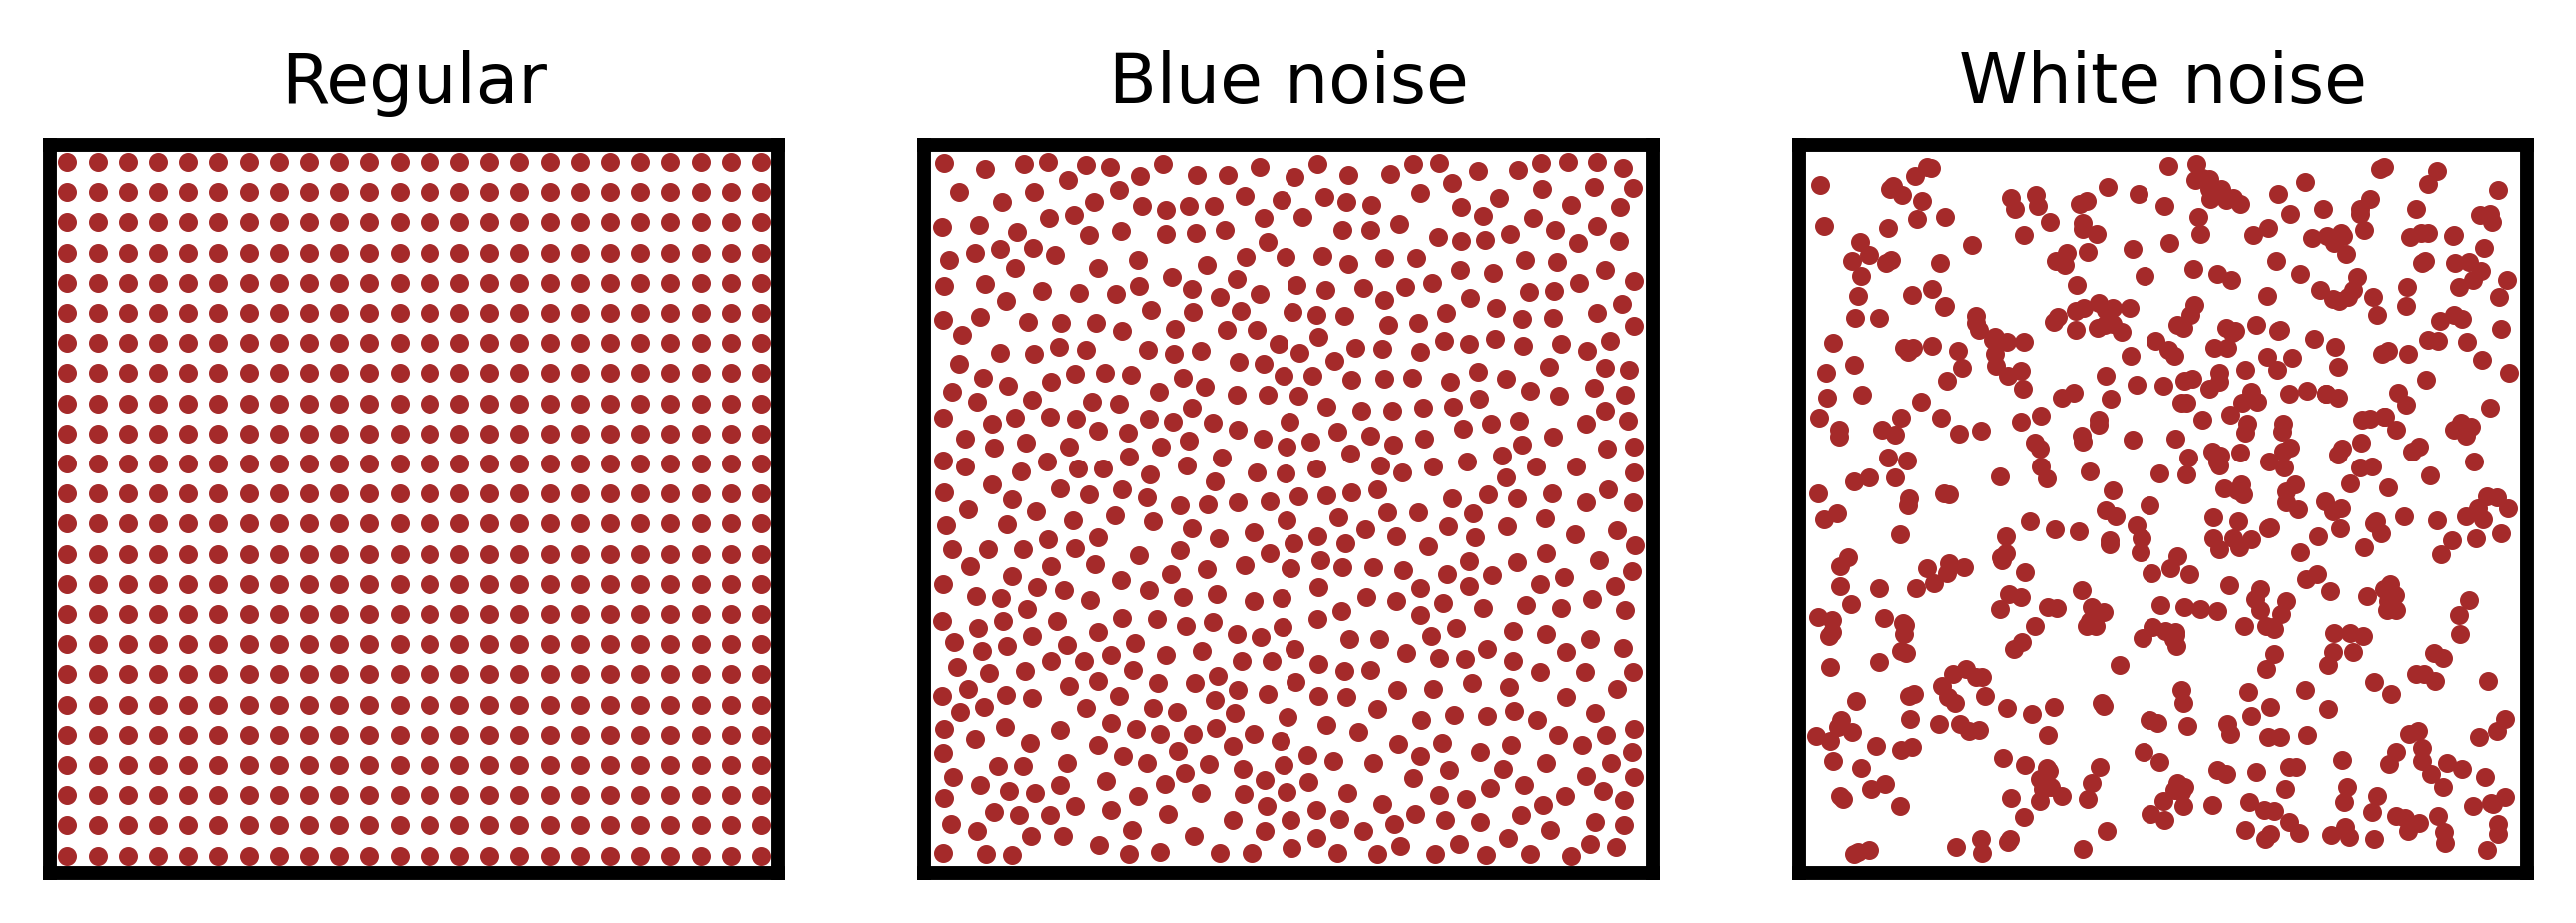
\includegraphics[width=\textwidth]{distribution_plot.png}
        \end{minipage}
        \caption{Examples of the three kinds of input distributions. Each plot shows 24x24 inputs. Regular distribution places inputs evenly across the entire environment in a rectangular way. A blue noise distribution places inputs sequentially so each is placed as far away from previously placed inputs as possible, resulting in an even, unstructured distribution. White noise distribution places inputs randomly, and independent of all other inputs, so some locations produce more input activity than others.}
        \label{input_distribution}
    \end{figure}
    
    The blue noise inputs were generated by iteratively suggesting a number of uniformly, independently distributed 2d-points, adding the point that was the furthest from all previously added points to the added points, and repeating until the desired number of added points was reached. To allow for good spread, the number of suggested points was directly proportional to the number of existing points.
    White noise inputs were generated by getting the desired number of uniformly distributed 2d-points independently of each other.

    \subsection{Multi-Compartment Model} \label{MC Model}
    A multi-compartment model was briefly justified in section \ref{Considering BVC inputs}, as a way to include non-linear dendritic computations which were interesting for BVC-inputs. The most natural way to implement this in the Brian2, the simulation software used, was as a separate, non-spiking layer between the input-layer and the transition cell layer, and simulate the synapses from dendrites to transition cells as gap junctions (figure \ref{network_MC}). To test the model with non-spiking dendritic computation without the complexity from BVC-inputs, this multi-compartment model (MC Model) used place-like input cells as an intermediary step between the models in previous sections and a full BVC-input model.

    \begin{figure}[h]
        \begin{minipage}[b]{\textwidth}
            \subcaption{}
            \includegraphics[width=\textwidth]{network_MC.PNG}
        \end{minipage}
        \begin{minipage}[t]{0.35\textwidth}
            \subcaption{}
            \includegraphics[width = \textwidth]{dend-to-soma.PNG}
        \end{minipage}
        \hspace{0.1\textwidth}
        \begin{minipage}[t]{0.54\textwidth}
            \caption{A multi-compartment model of the transition cell. (a) As opposed to models described in section \ref{Rect input} and \ref{Rand input}, the spiking transition layer soma does not receive spatial inputs directly - instead, spatial inputs synapse onto non-spiking dendrites, which conduct the voltage nonlinearly to the transition cell soma. In this model, a conductance parameter is the learning variable. (b) A representation of a single transition cell in the multi-compartment model. Each transition cell soma (right) receives inputs from a high number of dendrites (left). Dendrites can receive either place-like inputs or multiple BVC-inputs.}
            \label{network_MC}
        \end{minipage}
    \end{figure}

    To justify the two-layer neuron model with dendrites and soma as a multi-compartment model, the dendrites had the following properties: they only synapsed onto a single transition cell body, were non-spiking, and the dendrite-to-soma connectivity was modelled as a gap junction, as in \parencite{Alabi2022}. In this model, each dendrite only received input from a single input neuron, to simulate the place-oriented dendrite. Each dendrite had a voltage-parameter that would increment by a factor \(w\) when receiving inputs, and decaying to 0 over time (equation \ref{key5}):
        \begin{equation}\label{key5} v_{den}(t + 1) = v_{den}(t) + e^{-(v_{den}(t))/\tau} + \sum_{0}^{i} (w \cdot i(t-delay)) \end{equation}
    
    This resembles \ref{key2}, but does not have the option of setting voltage to 0 above some threshold, as the dendrite is non-spiking. In terms of inputs, with place-based inputs, each dendrite would only receive input from one input neuron. The weight \(w\) would be a hyperparameter, not changing during a simulation, and was equal for all dendrites.
    
    Based on this, the grid cell's voltage was determined by the following equation \ref{key6}. 
        \begin{equation}\label{key6} v_{soma}(t + 1) = \begin{cases} 0, & \text{if } v_{soma}(t) > \text{threshold or refractory}\\
        \sum_{i}^{} c_i \cdot tanh(v_i), & \text{otherwise} \end{cases}\end{equation} 
        
    Here, the nonlinear function \(tanh(v_i)\) gives the dendrite a softmax-like behavior, so the dendrite at anytime is either activated or not, dependent only on its internal voltage-parameter. \(v_i\) is the voltage of dendrite \(i\), \(c_i\) is the corresponding dendrite conductance, reflecting how effectively the dendrite's voltage affects the grid cell voltage. The learning rules \ref*{key3} and \ref*{key4} is here learning over conductances (\(v_i\)) instead of synapse weights, but is otherwise identical.

    With this network structure, simulation times were significantly higher than with direct connection between input cells and transition cells, because the number of dendrites was the product of the number of input cells and the number of transition cells. This limited the amount of time spent on this and subsequent models.

    \subsection{Boundary vector cell inputs} \label{BVC Model}
    The multicompartment model described above was modified so a dendrite received a set of BVCs as inputs instead of place-like cells. The softmax function was tuned so receiving only one or a few BVC-input would not ellicit any dendrite activity.

    This was begun in a simplified version, in which BVCs responded preferentially to one of the four cardinal directions, north, east, south or west, and with evenly distributed preferred distances. Then, each dendrite received a pair of orthogonal inputs, one from a BVC oriented to the northern or southern wall and one to the eastern or western wall, and the BVCs were carefully paired to give the dendritic tree an evenly spaced, rectangular input field. The activation function for a BVC was simply the distance to the wall in the preferred direction, converted linearly to temporal delay.
        
    While the equation for dendritic voltage was the same (equation \ref{key5}), the softmax-function for somatic depolarization in equation \ref{key6} was replaced with a hard step-function to reduce simulation times (equation \ref{key7}):
    \begin{equation}\label{key7} v_{soma}(t + 1) = \begin{cases} 0, & \text{if } v_{soma}(t) > \text{threshold or refractory}\\
        \sum_{i}^{} c_i \cdot (v_i > v_{threshold}), & \text{otherwise} \end{cases}\end{equation} 
    
    Compared to equation \ref{key6}, the dendritic conductance \(c_i\) was multiplied by a boolean which is 1 only for voltages above a threshold, \(v_{theshold}\). Considering that each dendrite only received two BVC inputs, \(v_{threshold}\) was typically between 1.2 and 1.5 times the fixed BVC-to-dendrite weight, so a dendrite needed both inputs in short succession to pass the step-function threshold.

    This also necessitated a change in the STDP-learning rule, since \(a_{pre}\) would increment not when the dendrite received an input, but when it passed the threshold \(v_{threshold}\).

    This model is structured to deliberately convert BVC-inputs to a dendritic tree with activity that resembles the model described in section \ref{Rect input}: rectangular inputs by carefully pairing orthogonal BVCs on dendrites, and a dendritic model that has replaced a soft-max learning rule with a step-function. Despite these simplifications, which might be justified as a proof of concept for BVC-inputs, this model did not yield gridlike transition cells like the previous models, halting further exploration.

    \subsection{Other network models} \label{Other Models}

    A few other network structures were tried apart from the methods above, but were not explored further because they were considered unsuitable. This section will describe the incentives behind these structures, and how they work.

    \subsubsection{Rate coded inputs} \label{Rate input}
    One structure was designed as an alternative to using phase-coded inputs described in section \ref{Rect input}. The model still relied on dense inputs, so in each position numerous inputs would be active, but their activity was rate-coded. Input cells here were modelled as LIF-neurons, so their voltage would decay to some base-value if the cell was not spiking or receiving inputs. To simulate rate-coded input activity, each input cell's base-voltage was frequently updated depending on animal position. For relevant spatial inputs, the base-voltage would end up above threshold, leading to spiking. Upon spiking, the voltage was reduced to a value below threshold, and remain there for a short refractory period, before again being affected be the depolarization towards the base-value.

    For a rate-code like this, a transition cell provided a feedback-signal to the input layer after spiking, which was tuned to only activating input cells that were close to threshold by that time. Coupled with a STDP learning rule, this network structure allowed transition cells to activate the surround-inputs themselves, which would force a post-pre spike timing, leading to dissociation. A challenge with this model was keeping the input structure stable, because the high firing rate center-inputs frequently would activate shortly after transition cell firing and dissociate. However, with single-cell networks, some measure of center-surround fields was achieved.

    This network structure was abandoned because having feedback-connectivity from transition cells to input cells was not in line with the TSS model.

    \subsubsection{Linear Summation BVC model} \label{LinnSummBVC}
    
    A simple model using direct BVC-inputs on transition cells modelled transition cells as simple LIF-neurons, integrating BVC-inputs and learning directly on the weights from these. Motivation for why this model was abandoned was given earlier, but this model was tested briefly nonetheless. One way to test the stability of the model was to artificially initiate the network with optimal weights for a hexagonal pattern, and see if it maintained the necessary firing dynamics. This was done by reverse-engineering weights, creating ideal firing patterns for each transition cell, by iterating over a 48 x 48 grid of the environment and increasing weights from inputs relevant to a firing position, decreasing weights from inputs that were irrelevant. This approach was not tried for any other methods, but when it failed to produce clear firing fields in the network, along with the arguments presented in section \ref{Considering BVC inputs}, this approach was not pursued further.

    \subsubsection{Linear Multi-compartment Models} \label{Lin MCModel}

    Models described in section \ref{MC Model} used a multi-compartment model of the neuron to allow dendritic computation to convert vector-based inputs to place-like inputs the transition cell could learn transitions on. In those models, the voltage in a dendrite was transformed to a voltage in the transition cell body through a nonlinear softmax-function. An alternative did not include the softmax transformation, instead modelling the transition cell body voltage as the sum of all dendrite voltages multiplied by conductances (equation \ref{key8}). \begin{equation}\label{key8} v_{soma}(t + 1) = \begin{cases} 0, & \text{if } v_{soma}(t) > \text{threshold or refractory}\\
        \sum_{i}^{} c_i \cdot v_i, & \text{otherwise} \end{cases}\end{equation} 
    Variables here have the same interpretation as in equation \ref{key6}.

    This model was not pursued for similar reasons as the model above: with BVC-inputs, a number of dendrites were slightly active with only a single BVC-input, producing similar dynamics (section \ref{LinnSummBVC}). Even if the learning rules were thresholded, so the STDP- and baseline-learning rules would only apply to moderately active dendrites, this errant activity would mean transition cells would activate too much in surround locations, losing circular firing fields.

    \subsection{Simulation software} \label{Sim software}
    
    All models and implementations can be found on github (Insert link here?), and while the simulation data is not available on github due to storage capacity, it is available upon request. All simulations were implemented in python, using the Brian2-library for its flexibility and easy implementation \parencite{Brian2}. With this framework, setting up simulations was straight forward, and allowed time-improvements such as only updating STDP-variables when relevant events occurred, not at every time step. Time steps were typically at 0.1 ms, which was also the minimal synaptic delay.
    
    Simulations with place-inputs used custom simulated trajectories, simulated with 10 ms time steps and a square environment. Position was treated like a continuous variable, with velocity and rotational velocity determined by normal distributions from one time step to the next. In simulations using boundary vectors, the external RatInABox library was used \parencite{RatInABox}. 
    
    From the trajectories, spatial inputs were calculated prior to simulations, using either position- or boundary information, and added to a brian2 spikeGeneratorGroup. The network state and weights were stored frequently during simulations.

    \subsection{Analysis} \label{Analysis}
    To investigate the firing properties of the network of transition cells, weights were frozen, and the activity of the network was sampled from each position in an even 48 x 48 grid across the environment. In simulations with input noise, each position was sampled 5 times, while they were sampled once without noise (figure \ref{analysis_plot} (a)). This gave data from the network state at one moment, which was subsequently stored as spike trains and then converted to histograms of spatial firing fields. Due to considerable computational time per sample, each simulation was typically sampled only every 5 minutes of simulated time.

    \begin{figure}[H]
        \centering
        \begin{minipage}[t]{\linewidth}
            \begin{subfigure}{0.32\linewidth}
                \subcaption{}
                \includegraphics[width = 0.9\linewidth]{analysis0.png}
            \end{subfigure}
            \begin{subfigure}{0.32\linewidth}
                \subcaption{}
                \includegraphics[width = 0.9\linewidth]{analysis1.png}
            \end{subfigure}
            \begin{subfigure}{0.32\linewidth}
                \subcaption{}
                \includegraphics[width = 0.9\linewidth]{analysis2.png}
            \end{subfigure}
        \end{minipage}
        \begin{minipage}[t]{0.38\linewidth}
                \subcaption{}
                \includegraphics[width = \linewidth]{analysis3.png}
        \end{minipage}
        \hspace{0.01\linewidth}
        \begin{minipage}[t]{0.59\linewidth}
            \caption{Visualization of different steps of analysis. (a) Artificial spikeplot from some cell. Each pixel represents one sampled position, and color indicates firing rate in that position. 1) Spacing is the distance between adjacent firing fields, from center to center. 2) Orientation is the angle between a wall and a line passing through adjacent firing fields. Due to the hexagonality of grid cells, this orientation is always between 0\(\degree\) and 60\(\degree\). 3) The phase can be understood as the offset from an environment corner to the closest firing field. In practice, another cell with similar spacing and orientation is used as base of comparison, instead of the environment corner (not shown here). (b) The autocorrelogram of the firing field. For a hexagonal firing field, this will also be hexagonal. Note that orientation and spacing is preserved, as the size of the autocorrelogram is twice that of the firing field. This hexagonal shape is always centered, making computations easier. (c) To compute gridness score, an annulus is taken from the autocorrelogram, so the first ring of fields are included. A highly hexagonal cell will have a 60\(\degree\) rotational symmetry, and antisymmetry at 30\(\degree\), 90\(\degree\) or 150\(\degree\) degree rotation. (d) Hypotheical firing fields at two times, and shuffled fields. The mean variance of the two fields is compared to the shuffled variance to measure temporal stability.}
            \label{analysis_plot}
        \end{minipage}
    \end{figure}
    
    Five primary variables were derived from each simulation, based on the spatial firing histogram: gridness score, spacing, orientation, phase distribution and temporal stability.
    
    The measure used to evaluate the hexagonality of the transition cells was primarily the gridness score. To find this score, an annulus was extracted around the center of the autocorrelation of the spatial firing fields of a sample (figure \ref{analysis_plot} (a) - (c)). The size of this annulus was estimated to find the first ring of maxima around the center. Using this annulus, gridness score was determined as \[gscore = min(a_{60\degree}, a_{120\degree}) - max(a_{30\degree}, a_{90\degree}, a_{150\degree})\] in which \(a_{n\degree}\) is the correlation between the annulus and itself rotated \(n\) degrees around its center.

    Gridness spacing was found by evaluating the gridness score with multiple estimations of annulus size, and determining values that gave the highest score (figure \ref{analysis_plot} (a) - (c)). Because of the discretization of space, multiple spacings would give similar scores, in which the middle value was taken.

    Orientation was determined only in cells with a positive gridness score. Orientation was determined as the angle between the horizontal line and the first maxima within the annulus, extracted similarly to in the gridness score (figure \ref{analysis_plot} (a) - (c)).

    Phase distribution was only evaluated for cells with positive gridness and an orientation between \(-5\degree\) and \(5\degree\), as this seemed to be dominant for most simulations (figure \ref{analysis_plot} (a)). In simulations with multiple cells passing these criteria, one cell was chosen at random as a basis for comparison. All other cells would be evaluated relative to this basis by doing a cross correlation, and finding the argument of the maximal value. To find all positions relative to the rhombus, the phase-difference was unsheared, so the rhombus would be rectangular. Then, phase differences could be reduced by a module-operation so all ended up within the same rectangle, and sheared again to be placed within the rhombus.
    
    Temporal stability was estimated by getting the variance in pixel-values in spike plots across time for each cell in the latter half of a simulation, and comparing the mean variances to the mean variance of shuffled pixel values (figure \ref{analysis_plot} (d)). This approach was enabled by the sampling scheme, in which each location in the environment was sampled equally at even time points. Shuffling the spike plots represented the expected temporal stability if there would be no correlation from one timepoint to the next, while a lower variance would imply a positive correlation of firing fields from one time to the next.

    \newpage
    \section{Results} \label{Results}

    \subsection{Defining Typical Parameters: a Standard Model} \label{Standard model}
    Several models were tested in this work. In most of these, overall network structure was kept the same, varying instead on certain parameters that were perceived as critical: the distribution of inputs, inhibition delay, the number of transition cells in a network and the role of noise in the spatial inputs. In addition to these variants, this section will show results from a multi-compartment model with non-spiking dendrites, both with place-like inputs and boundary vector cell inputs. Several hyperparameters could not be explored in detail due to the models' computational demand. In that light, this section will describe typical parameters of one model, and some of the considerations made in setting some of the parameters. This set of typical parameters ends up describing a standard model, which will be used as a baseline for comparison in the rest of the work. This model was chosen as the base model for comparison because it is closest to previous TSS simulations \parencite{Waniek2017}.

    Table \ref{param_table} shows a typical set of hyperparameters, partially chosen to be biologically plausible, but some sets of parameters were calibrated in order to achieve a wanted dynamic. Since the input was phase-coded relative to theta, weights and spiking threshold were set so the first transition cell would spike typically about halfway between the first input and the phase-delay cutoff. This was thought to encourage even center- surround fields under a STDP learning rule. Inhibitory delay was set to give a brief window for other cells to fire, and is probably shorter than expected biologically \parencite{Buetfering2014}. The apost, apre and baseline was set up to work in conjunction so potentiation and depression would approximately balance each other out, according to equations \ref{key3} and \ref{key4}. The standard model also assumed zero noise in the input phase delay for simplicity.

    \begin{table}[H]
        \caption{Example parameters for simulations. The parameters are partially chosen for biological plausibility, and partly adapted to achieve desired firing dynamics.}
        \begin{tblr}
            {
            colspec = {X[c,h]X[c]},
            stretch = 0,
            rowsep = 6pt,
            hlines = {black, 1pt},
            vlines = {black, 1pt},
        }
        
            \textbf{Parameter} & \textbf{Value} \\
            \# Transition cells & 13\\
            \# Inputs & 576 (24x24) \\
            Theta rate & 10 Hz \\
            Phase-delay cutoff & 20 ms \\
            \(\sigma\) & 0.012 \\
            \(\mu\) & 0 \\
            Transition cell threshold & 1.0 \\
            Transition cell \(\tau\) & 10 ms \\
            \(w_{max}\) & 0.14 \\
            \(w_{init}\) & uniform[0-0.75 \(\cdot w_{max}\)] \\
            \(A_{pre}\) & 0.01 \\
            \(A_{post}\) & -0.007 \\
            \(\tau_{pre}\) & 8 ms \\
            \(\tau_{post}\) & 80 ms \\
            Baseline & 0.005 \\
            Inhibitory delay & 0.6 ms \\
        \end{tblr}
        \label{param_table}
    \end{table}

    The simulations were run on a simulated trajectory, as described in the methods, using a one by one meter square environment. While weights and parameters were stored mid-simulations, data was also extracted from each model by sampling each position in a grid after freezing learning. Figure \ref{reg_spike} shows sampled cell activity over time in the standard model for seven cells in the same simulation. 
    
    
    \begin{figure}[htbp]
        \centering
        \includegraphics[width = \linewidth]{reg/spike.png}
        \caption{Sampled activity from seven transition cells in the same network throughout a simulation. Each plot represents activity in the same 1 x 1 m environment, subdivided into a 48 x 48 grid in which each position was sampled for a single theta cycle. Learning was disabled during sampling. Bright spots in the plots represent locations in which a transition cell was active, and each plot is smoothed with a gaussian filter. This sampling method is used for all models, although the number of samplings per position depended on noise levels.}
        \label{reg_spike}
    \end{figure}
    
    Clearly, transition cells typically develop center-surround fields quickly, evidenced already after 5 minutes of exploration from random initial activity patterns.

    Five primary variables were quantified about transition cell activity, all using these spike plots. The most central is gridness score, which quantifies the degree to which the firing fields are hexagonal. When finding grid cells in recordings of cell population, a way to qualify cells is by thresholding this score \parencite{Sargolini2006}.
    
    The three main variables for looking at grid cell populations were also used for transition cells in these simulations to compare with experimental data: grid spacing, orientation and phase distribution.
    
    Finally, a measure of temporal stability informs about whether the network converges to some state or is shifting. See section \ref{Analysis} for computational details.
    
    The following sections will outline results according to these five parameters for ten models: The standard model with parameters outlined in table \ref{param_table}, two models with similar parameters but different spatial input distributions (blue noise and white noise distributions, see figure \ref{input_distribution}), two models with a larger transition neuron network (23 and 37 cells), a model with minimal inhibitory delay (0.2 ms, but referred to as 'no delay', see section \ref{Rect input}) and three models with added input noise.
    
    Input noise occurred in the phase-delay of the input. Each theta cycle, each input had an expected delay depending on its spatial relevance relative to the animal's current position. The actual delay was modelled as normally distributed around this delay, with standard deviations of 1, 2 or 4 ms. All maintained a 20 ms temporal window each theta cycle.

    The tenth model is a multi-compartment model with parameters similar to the standard model, referred to as the MC Model (see  section \ref{MC Model}). This model also used place-like inputs, but these inputs synapsed on non-spiking dendrites, each dendrite only receiving inputs from one input cell, and each dendrite subsequently affecting a single transition cell's spiking in a gap-junction-inspired way.

    Each of the ten models was tested in 30 simulations on the same trajectory, and sampled every five minutes across the 95-minute simulation. Figure \ref{all_spikes} shows a randomly chosen 95th minute sample from each model, showing that each model produced isolated firing fields, but not necessarily high levels of gridness.

    \begin{figure}[H]
        \centering
        \includegraphics[width = \linewidth]{all_spikes.png}
        \caption{Spike histograms sampled after 95 minutes simulated time for all ten models compared in this work. Notice that although not all models are equally gridlike, all show clearly isolated firing fields, as predicted from a STDP center-surround learning rule.}
        \label{all_spikes}
    \end{figure}

    \subsection{Gridness scores in the different models} \label{Gscore}
    
    The central question to this work was whether the network structure and learning rule described in the methods section could produce transition cells with a hexagonal firing patterns, which can be quantified by the gridness score. This gridness score was always computed on spike plots such as those shown in figure \ref{reg_spike}. Figure \ref{gridness_plots} (a) shows final mean gridness scores for each simulation after 95 simulated minutes, grouped by model, while figures \ref{gridness_plots} (b)-(e) show the temporal development of gridness scores in the ten models sorted in groups.
    
    \begin{figure}[H]
        \centering  
        \begin{minipage}[b]{1\textwidth}
            \centering
            \subcaption{}
            \includegraphics[width=\textwidth]{model_comparison/model_comparison_gscores.png}
        \end{minipage}
        \begin{minipage}[t]{1\textwidth}
            \begin{subfigure}{0.5\textwidth}
                \subcaption{}
                \includegraphics[width=0.98\textwidth]{model_comparison/line_plot0.png}
            \end{subfigure}
            \begin{subfigure}{0.5\textwidth}
                \subcaption{}
                \includegraphics[width=0.98\textwidth]{model_comparison/line_plot1.png}
            \end{subfigure}
            \begin{subfigure}{0.5\textwidth}
                \subcaption{}
                \includegraphics[width=0.98\textwidth]{model_comparison/line_plot2.png}
            \end{subfigure}
            \begin{subfigure}{0.5\textwidth}
                \subcaption{}
                \includegraphics[width=0.98\textwidth]{model_comparison/line_plot3.png}
            \end{subfigure}
        \end{minipage}
        \caption{Gridness scores for ten model types. (a) Each scatter point represents mean gridness in one simulation after 95 minutes simulated time. Bars are means across all simulations for one type. (b-e) Loosely grouping the model types into four or five main categories. Colors are maintained from (a). (b) The multi-compartment (MC) model shares important parameters with the standard model; they both have networks of 13 transition cells, no input noise and rectangularly spaced inputs. The standard model seems to outperform the MC Model, but both show clear gridness. (c) Models receiving inputs from a blue noise distribution have approximately equal gridness to the standard model, while transition cell networks receiving white-noise inputs do not seem to have the same development. (d) Transition cells exhibit clear gridness both with minimal inhibitory delay and with different network sizes. While a network of 23 transition cells see the same gridness as the standard model, 37 transition cells have a somewhat reduced gridness. Without inhibitory delay, gridness is also reduced, and less stable. (e) While simulations with normally distributed input noise and std 1 or 2 ms have gridness comparable to the noiseless standard model, a std of 4 ms in input noise is not as robust.}
        \label{gridness_plots}
    \end{figure}
    
    While the standard model produced highest mean scores, multiple other configurations were comparable. Transition cell networks that received blue noise-distributed inputs, had 23 transition cells, or 1 ms noise yielded similar gridness, and developed approximately equally quickly. The multi-compartment model also had high gridness, but lower than the afore-mentioned groups, which was also the case for simulations with 37 transition cells, minimal inhibition delay or 2 ms noise. Finally, white noise inputs performed worse, while having some positive gridness, and 4 ms input noise did not produce stable hexagonality at all.
    
    Despite the differences in gridness, most cells across all simulations developed clear, isolated firing fields, and fired in multiple locations across the environment (see figure \ref{all_spikes}). To also have high gridness score, these firing fields should be bundled tightly to form hexagonal fields too, which might have separated some models from others.

    In all models, within-simulation variance in gridness was high, and virtually all simulations had some cells with a negative gridness score at all times (figure \ref{gscore_distribution}). Low gridness scores can be explained by grid shearing or firing fields that aren't evenly distributed across the environment, while negative scores tend to reflect rectangularity.

    \begin{figure}[H]
        \centering
        \begin{minipage}[b]{0.95\textwidth}
            \subcaption{}
            \includegraphics[width = 0.95\linewidth]{reg/distribution.png}
        \end{minipage}
        \begin{minipage}[t]{0.95\textwidth}
            \subcaption{}
            \foreach  \filename in {
                model_comparison/distribution_blue_noise.png,
                model_comparison/distribution_white_noise.png,
                model_comparison/distribution_no_delay.png,
                model_comparison/distribution_23grid.png,
                model_comparison/distribution_37grid.png,
                model_comparison/distribution_GJ.png,
                model_comparison/distribution_1ms_noise.png,
                model_comparison/distribution_2ms_noise.png,
                model_comparison/distribution_4ms_noise.png}
            {
            \begin{subfigure}{0.323\textwidth}
                \includegraphics[width=\textwidth]{\filename}
            \end{subfigure}
            }
        \end{minipage}
        \begin{minipage}[t]{\textwidth}
            \subcaption{}
            \includegraphics[width=\textwidth]{model_comparison/gscore_fluct.png}
        \end{minipage}
        \caption{Distribution of gridness scores in the different models. (a) Standard model gridness distribution with spike plot examples. Although the mean gridness of this model is considered high (above 0.6), most simulated networks contain cells with negative or low gridness score. Negative gridness is typically produced by rectangular patterns, as shown in the two leftmost spikeplot examples. The two middle examples show activity in cells with positive, but low gridness scores. To have a gridness score above 1, the hexagonal pattern must typically span the whole environment without shearing or rectangularity. (b) Gridness score distributions for the remaining nine models. (c) Proportion of cells with negative final gscore that also had negative gscore in all samples for the second half of the simulation. For most models, negative final gridness was not maintained across the entire simulation.} 
        \label{gscore_distribution}
    \end{figure}

    Interestingly, the distributions of grid scores can also reflect features of models with lower gridness scores. The models with minimal inhibitory delay have a wide variety in gridness, so some cells are highly gridlike and others highly un-gridlike, while models with white noise inputs have a higher mode, but rarely sees highly hexagonal cells (see row 1, column 2 and 3 in figure \ref{gscore_distribution} (b)). In the latter case, it is possible cells don't pack firing fields closely enough to develop high gridness, while in the former the between-transition cell competition might be too high to support large networks with high hexagonality.

    Across models, a minority of cells with negative gridness at the last sample time had maintained negative scores across the final half of simulations (figure \ref{gscore_distribution} (c)). This only exceeded chance levels of 5\% in three models, the two with larger networks and the MC model. For most models, this means that there might be some turnover in gridness, so at least some cells fluctuate between positive and negative scores over time. As demonstrated in section \ref{TempStab}, this doesn't necessarily mean that the transition cell firing fields are unstable in time, and is instead taken as an indication that small changes to firing fields can impact gridness score significantly. 

    \subsection{Orientation and phase distribution} \label{OrientationPhaseResults}

    According to experimental data, grid cells within a module align in orientation with a wall-angle offset of 7.5\(\degree\), which was also observed in previous simulations of the TSS-model with related learning rules \parencite{Stensola2015, Waniek2017}. Grid cells with similar spacing and orientation should have phases that are evenly distributed on the toroidal manifold the network is active on, as seen in \cite{Gardner2022}. 
    
    In this work, orientation was only computed for transition cells with positive gridness, and normalized to a value between 0\(\degree\) and 60\(\degree\). Phase distribution was only computed on cells that aligned with the dominant orientation of that model so phase distribution could be accumulated across multiple simulations, and normalized to a position within a rhombus of the environment that correspond to the unwrapped torus.

    In all simulations, the preferred orientation was around 0\(\degree\), which indicates that transition cells align firing fields preferentially parallel to one of the environment walls (figure \ref{orientation_phase_plot}). However, this wasn't a strong preference, at most one in four cells with positive gridness showed this directionality. Models with noise had less of an orientation preference, as was the case for models with no inhibitory delay. 
    
    \begin{figure}[H]
        \begin{minipage}[t]{\linewidth}
            \begin{subfigure}{0.2\textwidth}
                \includegraphics[width=\textwidth]{model_comparison/model_comparison_orientation_regular.png}
            \end{subfigure}
            \foreach \filename in {
                model_comparison/model_comparison_orientation_blue_noise.png,
                model_comparison/model_comparison_orientation_white_noise.png,
                model_comparison/model_comparison_orientation_23grid.png,
                model_comparison/model_comparison_orientation_37grid.png}
            {
            \begin{subfigure}{0.18\textwidth}
                \includegraphics[width=\textwidth]{\filename}
            \end{subfigure}
            }
            \begin{subfigure}{0.2\textwidth}
                \includegraphics[width=\textwidth]{model_comparison/model_comparison_phase_regular.png}
            \end{subfigure}
            \foreach \filename in {
                model_comparison/model_comparison_phase_blue_noise.png,
                model_comparison/model_comparison_phase_white_noise.png,
                model_comparison/model_comparison_phase_23grid.png,
                model_comparison/model_comparison_phase_37grid.png}
            {
            \begin{subfigure}{0.18\textwidth}
                \includegraphics[width=\textwidth]{\filename}
            \end{subfigure}
            }
            \vspace*{0.03\linewidth}

            \foreach  \filename in {
                model_comparison/model_comparison_orientation_no_delay.png,
                model_comparison/model_comparison_orientation_1ms_noise.png,
                model_comparison/model_comparison_orientation_2ms_noise.png,
                model_comparison/model_comparison_orientation_4ms_noise.png,
                model_comparison/model_comparison_orientation_GJ.png}
            {
            \begin{subfigure}{0.18\textwidth}
                \includegraphics[width=\textwidth]{\filename}
            \end{subfigure}
            }
            \foreach  \filename in {
                model_comparison/model_comparison_phase_no_delay.png,
                model_comparison/model_comparison_phase_1ms_noise.png,
                model_comparison/model_comparison_phase_2ms_noise.png,
                model_comparison/model_comparison_phase_4ms_noise.png,
                model_comparison/model_comparison_phase_GJ.png}
            {
            \begin{subfigure}{0.18\textwidth}
                \includegraphics[width=\textwidth]{\filename}
            \end{subfigure}
            }
        \end{minipage}
        \caption{Orientations and phases of all models. Transition cells prefer a 0\(\degree\) orientation in most models (1st and 3rd row), exceptions being the minimal inhibitory delay model and the model with most input noise. The standard model and blue noise input distribution model have the strongest preference, while either increasing network size or adding noise reduces the preference. To compute phase distributions, only transition cells with positive gridness and an orientation between -5\(\degree\) and 5\(\degree\) were considered. Within a simulation, one of the qualifying transition cells was chosen as a reference, and the dots show the other qualifying transition cells' phase relative to their reference (rows 2 and 4). This phase was computed as the offset of the peak relative to the center in the cross correlogram between the transition cell and the reference.}
        \label{orientation_phase_plot}
        
    \end{figure}

    One reason might be that simulated times were too short for transition cells to develop the 7.5\(\degree\) orientation preference seen in previous simulations, but based on 600 minute test simulations this did not seem to be the case.

    Relative phase distribution can only be investigated in simulations with minimally two cells sharing orientation, preferably more, and this was more common in larger networks. In networks with 23 or 37 transition cells, the phases is evenly spread, without clear signs of clustering (figure \ref{orientation_phase_plot} column 4 and 5 row 1). Notably, computing these phases was limited by the spatial resolution of the activity sampling, leading to rounding values.
    
    It was briefly checked if the 37-cell networks had a toroidal structure in the population activity, which would be expected for grid cells belonging to the same module. This did not yield interesting results, and while it should be not that those methods are created for larger networks, higher temporal resolution and rate-based network activity, it seems unlikely that networks with at most a third of the cells sharing orientation would have a highly ordered population activity structure. (move this, or give its own section? Also, should be in methods)

    \subsection{Gridness spacing} \label{Spacing}

    All ten models introduced in section \ref{Standard model} used, barring noise, the same threshold for which spatial inputs would activate in a given location. Given a STDP-learning rule that lets an active transition cell decorrelate from less relevant spatial inputs, it would be expected that this relevance threshold is critical for the size of transition cell firing fields. That does not, however, mean that all models would give transition cells with the same spacing.

    \begin{figure}[H]
        \centering
        \begin{minipage}[t]{\textwidth}
            \subcaption{}
            \includegraphics[width = \textwidth]{model_comparison/model_comparison_sigmas.png}
        \end{minipage}
        \begin{minipage}[t]{\textwidth}
            {
                \begin{subfigure}{0.126\textwidth}
                    \subcaption{}
                    \includegraphics[width = \textwidth]{model_comparison/spacing_spikeplot_simspam.png}
                \end{subfigure}
            }
            \hspace*{-0.01\textwidth}
            \foreach \filename in {
            model_comparison/spacing_spikeplot_noise_sims2.png, 
            model_comparison/spacing_spikeplot_noise_sims.png, 
            model_comparison/spacing_spikeplot_noise_sims3.png}
            {
                \hspace{0.01\textwidth}
                \begin{subfigure}{0.26\textwidth}
                    \subcaption{}
                    \includegraphics[width = \textwidth]{\filename}
                \end{subfigure}
            }
        \end{minipage}
        \caption{Grid spacing across ten models. This was computed as the spacing giving maximal gridness score for each cell after 95 simulated minutes. This was then filtered for cells with positive gridness. (a) Each dot represents the spacing in a single transition cell, sorted by model. Horizontal lines are model medians: for many models, the density is significantly higher close to the median that around.  Notably, while mean spacing is invariant on network size, adding noise increases median spacing. Models with white noise inputs also had increased spacing, but that might be caused by poor gridness overall. Moreover, the multi-compartment model had higher spacing than the standard model. (b - e) Spike plots of models with identical parameters apart from input noise. (b) The standard model, without input noise, has a mean spacing of about 32.5 cm. As opposed to models with noise, transition cells can fit four firing fields horizontally in a 1 x 1 environment (lower spikeplot). (c \& d) Models with 1 ms and 2 ms input noise have approximately similar mean spacing, at about 35 cm. (e) While 4 ms noise doesn't produce high gridness or clean firing fields, the average spacing is significantly larger than other models, with mean around 50 cm.}
        \label{spacing_plot}
    \end{figure}

    Curiously, while most models had highly similar spacing, which could be independent of input distribution and size of the transition cell layer (around 32 cm spacings), adding noise increased spacing, and it depended on amount of noise (figure \ref{spacing_plot}). This was especially true for the highest noise level tested, with mean spacing at 50 cm, while the 1 ms and 2 ms models had an approximately 35 cm spacing preference.

    \subsection{Temporal stability} \label{TempStab}

    Results from section \ref{Gscore} demonstrate that transition cells in many of the networks develop gridness, getting progressively more hexagonal with time(figure \ref{gridness_plots}). However, it is unclear if the fields converge on some stable configuration, or if they continuously shift throughout the simulation. Under the TSS model, transition cells with incremental, gradually improving hexagonality might be beneficial because transition cells also interconnect with place cells, so big changes in transition cell area will necessitate accurate changes in the connectivity between transition cells and place cells.

    \begin{figure}[H]
        \centering
        \begin{minipage}[t]{\textwidth}
            \subcaption{}
            \includegraphics[width = \textwidth]{model_comparison/model_comparison_temporal_stability.png}
        \end{minipage}
        \begin{minipage}[t]{\textwidth}
            \begin{subfigure}{0.347\textwidth}
                \subcaption{}
                \includegraphics[width = \textwidth]{model_comparison/sum_spikeplot_multi-grid.png}
            \end{subfigure}
            \foreach \filename in {
            model_comparison/sum_spikeplot_GJ_model.png, 
            model_comparison/sum_spikeplot_noise_sims3.png}
            {
                \hspace*{0.01\textwidth}
                \begin{subfigure}{0.297\textwidth}
                    \subcaption{}
                    \includegraphics[width = \textwidth]{\filename}
                \end{subfigure}
            }
        \end{minipage}
        \caption{Temporal stability of different models. (a) The measure used to quantify temporal variance was the mean variance in spiking activity from one sampled time to the next, normalized by the variance in the shuffled data. A one in this score would indicate that there is no linear correlation between spiking from one sample time to the next, five simulated minutes later, while values close to zero indicate a positive correlation. Input noise decreases temporal stability, while inhibitory delay increases it. Larger networks also show more resistance to change. (b - d) The 95 minute sample activity (row 1) and summed activity over all sample times (row 2) for two cells each of three different models. All three models have clearly defined regions of activity and inactivity in their 95th minute sample. The summed activity, however, shows that transition cells in the 37 transition cell model and the multi-compartment model have maintained firing fields over time, while the noise model has not. This is reflected in their corresponding temporal variance scores.}
        \label{temporal_stability_plot}
    \end{figure}

    To investigate this, a measure for temporal stability was used which tracks the transition cell activity in each of the sampled locations over time (figure \ref{temporal_stability_plot} (a)). The measure is a temporal correlation, in which the variance from one sample to the next, taken five simulation minutes later, is compared to the variance with shuffled data. This shuffled variance is used as a standard for no correlation, so a variance between 0 and 1 represents a positive temporal correlation, and variances above one is a negative correlation.
    
    A positive correlation is clearly expected, because the input weights at one sampling time will be correlated to input weights at the next sampling. Additionally, the STDP learning rule is expected to encourage a cell to associate to some place and keep firing there. As such, the measure doesn't clearly indicate what should be understood as high temporal stability. Looking at spike plots instead, showing mean firing rates in each sampled location over time, shows a clear difference between models with low and high temporal stability (figures \ref{temporal_stability_plot} (b) - (d)). Two randomly picked cells from three different models were chosen: the 37 transition cell model, which had the highest recorded stability, the 4 ms noise model with the lowest stability and the multi-compartment model as an intermediate one. The first row in each plot shows the activity at the final sampled time, 95 minutes, while the second row shows the summarized activity over all times. The 4 ms noise model shows comparably homogenous summed activity relative to the single-time sample, which is expected of models with low temporal stability. The other two models, on the other hand, show clearly peaked summed activity. This is taken as an indication that these models, and models with comparable spatial stability, produce transition cells that maintain their firing fields over time, and can represent spatial transitions stably.

    Temporal stability seems to predict prolonged negative gridness, as shown in figure \ref{gscore_distribution} (c). Despite the perceived benefit of temporal stability, it might also show inflexibility and a struggle to converge on hexagonal firing fields.


    \subsection{Boundary Vector Cell Inputs} \label{MCModResult}
    One goal of this work was to investigate the nature of spatial inputs. While previous sections describes how transition cells can obtain hexagonal activity with place cell-like inputs, the TSS model proposes that this input is conveyed to the transition cell soma through active computation in a dendritic tree \parencite{Waniek2020}. The spatial inputs given to this dendritic tree could have some other form, such as boundary vectors. Here, the dendritic tree is modelled as a multi-compartment model in which dendrites act as perceptrons, receiving some input and activating according to a softmax function to influence the transition cell body.

    The only model that has been presented so far in doing this was a highly simplified version, in which the spatial input was rectangularly distributed and place cell-like, and the dendritic layer was simply conveying this information directly to the soma in a non-spiking manner, as a proof of concept. This model performs similarly to the standard model, but lacks a little in gridness (sections \ref{Gscore} - \ref{TempStab}). An obstacle is that the addition of this intermediate dendrite layer increases simulation times signifcantly, so getting the right spiking dynamics as outlined in \ref{Standard model} is slow.

    Further effort was made to move from this to a model taking boundary vector cell inputs. If dendrites should take BVC-inputs and convert them to place-like activity regions, this should be done in accordance to the previous results. Most importantly, if each dendrite responds to a single, random location independent of all other dendrites, the resulting dendritic tree might have a white-noise-like input distribution, which has been suboptimal in previous simulations.

    With this in mind, the simplest BVC-model tried to replicate the rectangularly spaced inputs, so each dendrite received only two, orthogonal BVCs carefully tiled so each dendrite responds highly to a single position in a rectangular grid (figure \ref{BVC_input} (a) \& (b)). With this dual input, the dendrite stepwise activity would activate strongly when the input timing coincides, favoring places where both BVCs are equally far from their favored firing activity (figure \ref{BVC_input} (c)). This gave dendrites a diagonal cross-like firing field, which is different from the firing fields used in dendrites in the MC model.

    \begin{figure}[H]
        \begin{subfigure}{0.315\textwidth}
            \subcaption{}
            \includegraphics[width = \textwidth]{bvc_act.png}
        \end{subfigure}
        \hspace{0.02\textwidth}
        \begin{subfigure}{0.315\textwidth}
            \subcaption{}
            \includegraphics[width = \textwidth]{den_act1.png}
        \end{subfigure}
        \hspace{0.02\textwidth}
        \begin{subfigure}{0.315\textwidth}
            \subcaption{}
            \includegraphics[width = \textwidth]{den_act2.png}
        \end{subfigure}
        \caption{Boundary vector cell- and dendrite example activity during sampling. (a) In this model, all BVCs will align in one of the cardinal directions, giving them firing fields parallel to either the north/south walls or east/west walls. Distances were spaced linearly across the BVC population. (b) Dendrites would have an approximately circular firing fields at the intersection of their two input BVCs, if activity was limited to the first 10 ms of each theta cycle. (c) Across the entire time window, dendrites would activate in corners diagonal to their center of firing, places were their inputs would coincide late in the input window. This limits the similarity between this model and the models described in previous sections.}
        \label{BVC_input}
    \end{figure}
    
    Next to the place-preference of each dendrites in this model, an advantage is that the state of the network can be directly read out from the dendrite-to-transition cell weights, or their conductances, as it is known at the start of a simulation which dendrite should respond to which place (figure \ref{BVC_spikeplot} (b)). Although this model didn't develop overall positive gridness in test simulations, it did give transition cells with clear spatial firing fields (figure \ref{BVC_spikeplot} (a)). Although this does not allow definitive conclusions on BVC as possible input structure, this shows some promise for this kind of model. 

    \begin{figure}[H]
        \begin{subfigure}{\textwidth}
            \subcaption{}
            \includegraphics[width = \linewidth]{BVC_spikeplot.png}
        \end{subfigure}
        \begin{subfigure}{\textwidth}
            \subcaption{}
            \hspace*{0.01\linewidth}
            \includegraphics[width = 0.995\linewidth]{BVC_spikeplot_weights.png}
        \end{subfigure}

        \caption{Preliminary results from a simplified BVC-model (a) Time series of sampled spike plots. Although the development of hexagonality isn't convincing, there are spatially separated firing fields. Each transition cell receives inputs from 24 x 24 dendrites, similar to the MC Model, but these dendrites receive input from a pair of orthogonal BVCs. Values below final row are gridness scores of the corresponding firing histogram. (b) Dendrite-to-transition cell conductances from the bottom row in (a), sorted so each dendrite is placed in the intersection between the preferred firing fields of its two input BVCs.}
        \label{BVC_spikeplot}
    \end{figure}

    \newpage
    \section{Discussion} \label{Discussion}

    \subsection{What this model shows} \label{TheseResults}
    The goal of this work was to identify how biologically plausible simulations of transition cells of the TSS model match experimental observations of entorhinal grid cells. Although studies on grid cells are numerous, some key variables were emphasized. First, that the network structure and morphology is reasonably close to the observed grid cell networks in the medial entorhinal cortex (mECII), so the transition cells are interconnected via strongly inhibiting interneurons. Secondly, that the activity pattern of the transition cells fit some criteria: most importantly that their firing was sufficiently hexagonal to pass as gridcells, and then that their firing properties follow that of single grid cell modules with similar grid spacings, a 7.5\(\degree\) wall-angle offset, and were reasonably temporally stable. On a population level, the criteria were arbitrarily large networks, uniformly distributed phases and a toroidal structure in the population activity. Finally, the spatial inputs given to grid cells should plausibly exist prior to learning a given environment, for instance driven by boundary vector cells, as opposed to place cells.

    To match the TSS model, the transition cell layer would receive dense spatial inputs, and self-organize so each transition cell encodes as many spatial transitions as possible under a learning rule described in the TSS-model. This learning rule is based on two competing rules: first, that transition cells associate to central areas, where it encodes transitions from, to an annulus-shaped surrounding area where it encodes transitions to, and secondly that it tries to be active everywhere. This is a learning rule that leads, in theory, to optimally efficient transition cells.

    The results and networks described here fits a majority of these requirements: the learning rule is in line with the TSS model, and cells turn out as valid transition cells. This is coupled with networks that are reminiscent of the mECII grid cell network, which is characterized by strong lateral inhibition. It is not clear that grid cells get spatially modulated input that is phase coded based on its relevance, but the theta-oscillations seen in the mEC shows some evidence of rhythmic activity \parencite{Winson1978}. Importantly, the learning rule, given place-like inputs, produces transition cells with high levels of gridness, that share spacing across the population and show temporal stability (figures \ref{gridness_plots}, \ref{spacing_plot} and \ref{temporal_stability_plot}). This is true for different network sizes, with 13, 23 or 37 transition cells, although gridness decreased in the latter.
    
    It is unclear if this fall in gridness in 37 cell networks implies an upper limit in network size. Getting high gridness has often been a case of setting parameters well, and if the parameter space giving high gridness shifts from changing network size, that would not have been caught in the simulations ran here. One example of this parameter shift is the reason all simulations here uses 24x24 inputs: early simulations achieved the wanted dynamics better than for models with 48x48 inputs, although increasing parameter count should increase spatial resolution, not decrease it. In both these examples, running larger networks increased both simulation time, making smaller networks appealing. This is discussed further in section \ref{ParameterDiscussion}.
    
    This model proved reasonably robust to noise, although the model with a 4 ms std on input noise did not develop stable gridness. The obseration that transition cells developed bigger fields with noise might be interesting in this regard - it is possible that there is some ideal spacing for transition cells based on the environment size, because some number of activity fields is beneficial. Models with noise might benefi from a smaller receptive field, to fit this ideal size. However, this would only be the case in a spatially confined environment, which might not be evolutionary adaptive for rodents. Moreover, how noise increases spacing isn't explored, particularly in terms of the absurdly high spacings in the 4 ms noise model. This model did show more problems developing center-surround fields than others, which might explain both the spacing and the gridness.

    Looking at single cell characteristics, there are two primary questions left open from the results: first, that very few simulations produced cells with unvaryingly high scores, instead often containing cells with low or even negative gridness. Second, that while transition cells partly coorganized with a single orientation, there was no preference for the empirically supported 7.5\(\degree\) wall angle offset. Instead, transition cells aligned perfectly with the wall.

    Due to the universality of these problems - all models had large within-simulation variance in gridness score, and all models either preferred 0\(\degree\) wall angle offset or had no dominating orientation (figure \ref{orientation_phase_plot}), and little improvement in longer simulations in both - there is reason to think that something is missing structurally, and not just that the parameters are wrong. This has also been seen in other feedforward models, discussed in section \ref{Other model comparisons} and \ref{TSS model comparison}, but examples on changes that could be made is varying inhibitory strength, as is seen in CAN models, or stronger transition cell dissociation with an interaction learning rule, as in the previous TSS-simulations.

    While the models here supported networks of 37 transition cells, which developed reasonable gridness, cooriented with a 0\(\degree\) wall-angle offset and had uniform phase distribution, there was no evidence of population activity on a toroidal manifold. Existing literature shows how population activity within a grid cell module should represent the animal's position on a twisted torus \parencite{Gardner2022}. However, the best simulation for this kind of work would be a single 37-cell simulation in which ten cells had positive gridness and an approximate 0\(\degree\) wall-angle offset, while the methods used to investigate this, inspired by \cite{Gardner2022}, depend on hundreds of grid cells. This would be an interesting line of study, but requires this model to be scaled up significantly. 

    The toroidal population structure also implies that the transition cells would maintain relational firing across environments - this could be investigated further by running simulations consecutively with the same cells. However, with uniformly distributed initial weights and non-discriminatory inhibition, there is no mechanism in the network that encourages this kind of coalignment. Additionally, new [unpublished?] observations suggest that the mEC grid cell network has a toroidal activity pattern even prior to any spatial exploration.

    In sum, this implies that there are missing elements in the models, including the standard model presented in \ref{Standard model}. Its simplicity is an argument in its favor, but there is work remaining in making the transition cell network coalign in a single module, which is clearly the case in the mECII. That the network should have the structural property prior to exploration means that the network structure probably should be changed.

    Next to matching with experimental data, significant effort was made in this work to see how spatial inputs influence the transition cell network. An early goal was to use BVCs as inputs, and while this was never done convincingly here, some ideas at how this could be done was explored. These will be explored in section \ref{Future: BVCs}.

    \subsection{A word about parameters}\label{ParameterDiscussion}

    As has been alluded to frequently throughout this work, simulating neural networks, and maybe particularly spiking neural networks, includes setting numerous parameters (see table \ref{param_table}). Understanding what each parameter does is a tall order, considering their numerous interactions, which was for instance shown when networks with minimal inhibitory delay gave positive results, countering the hypothesis (figure \ref{gridness_plots}). Tuning hyperparameters to make learning rules that balance the incrementation and decreasing of weights required time and experimentation - in many networks, activity would fizzle out due to an overreactive dissociation. Increasing or decreasing network size, number of inputs or spiking threshold changed simulation results thoroughly. Even if time hadn't been a constraint on this thesis, testing all parameter combinations would have been intractable.

    With this in mind, it is worthwhile to stress that the majority of the results shown here are based on relatively little experimentation with parameters. The model with white noise distributed inputs was more closely tested than the standard model and blue noise distributed input models, because of the perceived convenience of completely unstructured inputs. The fact that this model didn't produce high gridness nonetheless, isn't a conclusive proof that it's impossible, but rather a sign that it's implausible - getting a transition cell network to achieve gridness is probably easier with more homogenous spatial input distributions.

    This should influence how results from models like this are interpreted. Occam's razor suggests that simple models should be preferred. Spiking neural networks are hardly simple, because of the number of parameters, so a useful measure can instead be the range of parameters that show the wanted properties. It might be interesting to test different learning-parameters, to judge the relative importance of the STDP-rule versus the baseline rule. Instead, all model results here might better be taken as proofs of concept.

    \subsection{Comparison to existing grid cell models} \label{Other model comparisons}

    To the writer's knowledge, this is the first grid-cell model using phase-coded spatial inputs, an input structure that links mECII grid cells to the theoretical transition cells of the TSS-model. From the perspective of TSS, phase coding the spatial relevance gives transition cell information about center- vs surround fields. The transition cell uses this information to divide the environment into regions it encodes transitions from, and regions it transitions from. In terms of biological plausibility, phase coding aligns with spike timing dependent plasticity as a learning rule that has been experimentally verified in the brain. A strength of the model is that it does not rely on normalizing spike rates across the cell population or using implausible learning rules such as backpropagation through time (BPTT), which can be found in other grid cell models \parencite{Kropff2008,Sorscher2023}. Integrating spike timing and phase coding into a learning rule is an advantage biological, continuous time networks have, and might be central in understanding the brain beyond artificial neural networks. That being said, the upstream structure producing phase-coded inputs to transition cells is not yet seen in the brain, and might depend on advanced dynamics. 

    The models developed here are not pure feedforward models, because of the lateral inhibition between transition cells, but they share many features with other models in this group. The benefit of learning gridness through association and dissociation to spatial inputs, as feedforward networks tend to do, is that the grid cell activity is less sensitive to drift \parencite{Mulas2016}. To some extent, this was reflected in the temporal stability shown in this work.

    However, grid cells in feedforward models have some typical characteristics that do not fit experimental data, and that is true for this model too. Firing rate adaptation models required ad-hoc implementations to make grid cells co-orient, using excitatory recurrent connectivity \parencite{Barry2006,Si2013}. Although the model presented in this work showed some degree of preferred orientation, altering lateral connectivity might be necessary to strengthen this preference and align the cells with the theoretical 7.5\(\degree\) wall angle offset, which was seen in previous transition cell simulations \parencite{Waniek2017}. 

    Another feed-forward model, combining inhibitory and excitatory inputs to the grid cells, gave a gridness score distribution similar to the one seen in this work \parencite{Weber2018}, and the cells had similar firing fields - although firing fields developed, shearing or rectangularity reduced scores. Possibly, it is the competition across the population that makes some cells struggle to develop hexagonality, but this is unknown.

    Both the wide distribution of gridness scores and the lack of a wall angle offset can be addressed by changing the lateral connectivity between transition cells in the network, for instance by changing the role of inhibition. A goal would be to implement these models in larger networks, comparable to the neural recordings in \parencite{Gardner2022}, and investigate if structured inhibition can place population activity on a toroidal manifold. Examples would be to make transition cells inhibit other transition cells with varying strength, or with different inhibitory delays. Getting a toroidal population activity would presumably imply co-orientation, and possibly a narrower distribution of gridness because firing fields for different transition cells would correlate more strongly. Whether such networks would preserve mean gridness score and uniform phases remains to be seen.
    
    An implication of this lateral connectivity would be that the transition cell population is a continuous attractor network. One rationale for this, under TSS, is that increasing mean gridness would make transition cells encode more transitions, on average. Although this work implies that transition cells can bundle a high number of spatial transitions with the networks used here, it would be in line with the TSS model if simple changes to network connectivity would improve transition-bundling further. Finding a proper union between the toroidal manifold of the grid cell network and the transition cells of TSS might require theoretical work on how transition cells ideally should coorganize in networks.
    
    \subsection{Comparison with existing TSS simulations} \label{TSS model comparison}

    Transition cells, under the TSS-model, learn spatial transitions by associating to spatial information related to center-regions they encode transitions from, and dissociating from spatial information related to surround-regions, which they encode transitions to. A mechanism to support this is dense sampling, in which, in any given position, both spatial information from the places corresponding to center and the surround will be available \parencite{Waniek2020}. This lets the transition cell acquaint to all spatial information, which is necessary to subsequently represent spatial transitions. Transition neurons also communicate laterally with inhibition, to discourage overlapping fields and representing the same transitions. 
    Prior to this work, all simulations of spatial learning under the TSS-model had unresolved questions that needed to be answered to be applicable in a biological network: how could a high number of transition neurons coexist in the network, and what would a biologically plausible learning rule look like? In the original simulations, inhibition times were instant, rate of learning was modulated by the number of inputs to account for edge effects, and the only input structure tested was one with a rectangular distribution.
    Compared to this, this work is a decisive step in the direction of biological plausibility, showing high degrees of gridness in larger networks, as well as uniform phase distributions. Although this work did not show explicit hexagonality with BVC-inputs, it showed gridness with different input distributions, a smaller number of dendrites (576 vs 2304) and only velocity-based learning rate modulation.

    Existing simulations of the TSS model had a third learning rule, an interaction rule, in which transition cells dissociated from spatial information whenever another transition cell activated first \parencite{Waniek2017}. This learning rule wasn't implemented here because it wasn't clear how - one plausible alternative is that receiving inhibition would decrease weights, but this was technically difficult to implement with the simulation library used, and would have increased simulation times. However, a learning rule like this might encourage faster convergence and a wall-angle orientation closer to the 7.5 degrees that might be expected, due to its high number of packed center-surround areas. On the other hand, this learning rule might also strain the network more in terms of size, because it discourages overlapping fields.

    \subsection{The future: benefits of BVCs, biological plausibilities etc} \label{Future: BVCs}

    Considering that optic flow can explain boundary vector cell activity from pure visual inputs, a network producing gridlike cells from BVC-inputs is desirable because it explains how spatial transitions can be learnt from sensory information available at the time of exploration \parencite{Raudies2012}. Under certain conditions, it might also extrapolate to other vector-based inputs, such as object-vector cells, given that these cells can also be modeled from optic flow, and that there is a sufficient number of landmarks to triangulate positional information from. Although this work by no means is conclusive on the nature of such a network, nor any concrete data on the BVC-to-transition cell network, it provides some predictions at what such a network should look like.

    Importantly, because most BVCs will be active in both the center- and the surround-region of the transition cell (see section \ref{Considering BVC inputs} and figure \ref{BVC_input} (a)), linear summation of all boundary vector cell activity is unlikely to yield effective transition cells. Instead, some nonlinear process is necessary to allow transition cells to respond to BVCs in some locations, and not in others. In this work, the mechanism that supports this is dendritic computations, in which each dendrite receives a subset of BVC-inputs, and the transition cell in practice can learn on each dendrite, instead of individual inputs. This idea followed both experimental data on superlinear activation of pyramidal grid cell dendrites \parencite{Schmidt-Hieber2017}, as well as a model using dendritic computations to explain place cell remapping \parencite{Alabi2022}. In this model, each dendrite adapted to some place in some environment, and context-signals would inhibit all dendrites except the one governing the current environment. This allowed the place cell to remap orthogonally.

    Using the same idea in this work, so each dendrite would represent some location in the environment, the learning variable was the dendrite conductance, and not synaptic weights. This isn't grounded in experimental observations, but rather because it contributed to model simplicity in two ways: first, that this mimics models in which place-like spatial inputs synapse onto grid cells, such as the other models in this work. This clarifies comparison, because the learning variable always has the same functional role in the network, as place-input to grid-cell weights. Secondly, although not directly explored here, one way of self-organizing BVC- to dendrite-connectivity is by randomly connecting a superfluous number of BVCs on each dendrite, and pruning unnecessary connections so the dendrite activates in only one or a few places. Differentiating between these two kinds of learning - BVC-to-dendrite and dendrite-to-grid cell, was thought to make these processes easier to distinguish. 
    This model provides the testable hypothesis that 1) dendrites of either stellate or pyramidal mECII grid cells will exhibit place-like activity fields during traversal of familiar environments, and 2) only depolarization in certain grid cell dendrites, those responding to places within one of the firing fields of the grid cell, contribute to somatic depolarization and grid cell spiking.

    That being said, while learning can occur in dendrite-to-grid cell conductances, these models don't depend on it. Alternatively, the STDP-learning signal must be transmitted to all postsynapses in the dendrite, in which all the weights will be changed indiscriminately, except possibly those pruned by mechanisms described in the above paragraph. In this case, it is also possible that all dendrites end up with place fields within the grid pattern.

    One of the most direct predictions from this work is that in the case of such a dendritic input tree, the distribution of place-like inputs to the grid cell should be relatively evenly distributed spatially. With LIF model neurons, it might be more difficult to converge on proper gridness when inputs have place fields that are uniformly and independently distributed. A more even distribution, such as a blue noise pattern, is for instance seen in the layout of cones in the human retina \parencite{Yellott1983}, but to make dendrites activate in a blue noise pattern would require some mechanism, for instance by making them disassociate from each other.

    Some further challenges underlie the model relying on an expansive dendritic tree as a hidden layer between vectorized inputs and grid-like transition cells. Not only is the number of dendrites quite high compared to both stellate and pyramidal principal mECII cells \parencite{Klink1997}, but if each dendrite should correspond to one location, the required number of dendrites required would need to scale linearly with the number of places visited. If inspiration is again taken from what is known of hippocampal place cells, some kind of context modulation or remapping might help explain this, but significant work is required to highlight how this would work. With BVC-input, the same dendrite would in principle respond to the same place in multiple environments, as long as the boundary information is similar, so each dendrite could be reused across contexts as long as conductances could be modulated across environments. Prior to exploring this in the engineer-like simulations like this work has done, this question should be investigated in a theoretical framework.
    It is, however, in the spirit of the TSS to assume that the dendrites of a transition cell serves some computational purpose, and does this well.

    \newpage
    \section{Conclusion}
    In the process of exploring areas of biological implausibility in the Transition Scale-Space model, this work has demonstrated the power of biological neurons integrating continuous time and space. A criticism of the TSS model was that its simulations were implemented with for instance instant inhibition and backpropagation-based navigation, which require computational resources that might not be available in the brain. Results from this work indicates that transition cells can be learnt from boundary vector cell activation using phase-coded activity, delayed inhibition and dendritic computation, resources that have established roles in the brain but not used in perceptron in today's artificial neural networks. In parallel work, changing delay was tested as a potential alternative to the backpropagation used in Dijkstra's algorithm. 
    
    While results are promising, there are multiple areas of further development. First is exploring how and why a transition cell population should activate on a torusoidal manifold. Establishing the full link from BVCs to transition cells, not to say visual inputs to transition cells, would be central for the model. Finally, there is a long way left to test if spike delay can provide the necessary information for a biological alternative to backpropagation.

    \printbibliography{}

\end{document}